\documentclass[12pt,a4paper,oneside]{report}

\makeatletter
\@ifundefined{XeTeXversion}{
  \@ifundefined{luatexversion}{
    % pdfLaTeX compilation mode
    \usepackage[utf8]{inputenc}
    \usepackage[vietnamese]{babel}
    \usepackage[T1]{fontenc}
    \usepackage{tgtermes}
    \usepackage{tgheros}
    \usepackage{tgcursor}
  }{
    % LuaLaTeX compilation mode
    \usepackage{fontspec}
    \setmainfont{TeX Gyre Termes}
    \setsansfont{TeX Gyre Heros}
    \setmonofont{TeX Gyre Cursor}
  }
}{
  % XeLaTeX compilation mode
  \usepackage{fontspec}
  \setmainfont{TeX Gyre Termes}
  \setsansfont{TeX Gyre Heros}
  \setmonofont{TeX Gyre Cursor}
}
\makeatother
\usepackage[left=3cm,right=2cm,top=2.5cm,bottom=2.5cm]{geometry}
\usepackage{setspace}
\setstretch{1.4}
\usepackage[final]{graphicx}
\graphicspath{{IMG/}}
\usepackage{float}
\usepackage{booktabs}
\usepackage{longtable}
\usepackage{tabularx}
\usepackage{array}
\usepackage{multirow}
\usepackage{amsmath,amssymb,mathtools}
\usepackage{xcolor}
\usepackage{enumitem}
\usepackage{listings}
\usepackage{fancyvrb}
\usepackage{caption}
\usepackage{subcaption}
\usepackage{tikz}
\usetikzlibrary{arrows.meta,positioning,shapes.geometric,fit,calc}
\usepackage{pgfplots}
\pgfplotsset{compat=1.18}
\usepackage{fancyhdr}
\usepackage{hyperref}
\usepackage[nameinlink,noabbrev]{cleveref}

\definecolor{viqablue}{HTML}{0B5FA5}
\definecolor{viqacyan}{HTML}{148BA8}
\definecolor{lightblue}{HTML}{EAF4FA}
\definecolor{lightgray}{HTML}{F3F4F6}
\definecolor{darkgray}{HTML}{374151}
\definecolor{E76F51}{HTML}{E76F51}
\hypersetup{
  colorlinks=true,
  linkcolor=viqablue,
  citecolor=viqablue,
  urlcolor=viqacyan,
  pdftitle={VIQA Nexus - Hệ thống hỏi đáp tiếng Việt},
  pdfauthor={Nhóm sinh viên NLP Summer 2026}
}

\pagestyle{fancy}
\fancyhf{}
\fancyhead[L]{\small VIQA Nexus}
\fancyhead[R]{\small NLP Summer 2026}
\fancyfoot[C]{\thepage}
\renewcommand{\headrulewidth}{0.4pt}
\setlength{\headheight}{15pt}
\setlength{\parindent}{1.2cm}
\setlength{\parskip}{0.25em}
\setlist[itemize]{leftmargin=1.8em,itemsep=0.25em,topsep=0.35em}
\setlist[enumerate]{leftmargin=2em,itemsep=0.25em,topsep=0.35em}
\captionsetup{font=small,labelfont=bf}
\renewcommand{\contentsname}{Mục lục}
\renewcommand{\listfigurename}{Danh mục hình}
\renewcommand{\listtablename}{Danh mục bảng}
\renewcommand{\arraystretch}{1.25}
\sloppy

\newcolumntype{Y}{>{\raggedright\arraybackslash}X}
\newcolumntype{C}[1]{>{\centering\arraybackslash}p{#1}}
\newcolumntype{L}[1]{>{\raggedright\arraybackslash}p{#1}}

\tikzset{
  block/.style={draw=viqablue,rounded corners=2pt,fill=lightblue,
    minimum height=1.05cm,text width=2.5cm,align=center,font=\small},
  smallblock/.style={draw=viqacyan,rounded corners=2pt,fill=white,
    minimum height=0.9cm,text width=2.05cm,align=center,font=\small},
  flowarrow/.style={-{Latex[length=2.5mm]},thick,draw=darkgray},
  groupbox/.style={draw=gray,dashed,rounded corners=3pt,inner sep=7pt}
}

\begin{document}

% ------------------------------------------------------------------
% TRANG BÌA
% ------------------------------------------------------------------
\begin{titlepage}
\thispagestyle{empty}
\begin{center}
\vspace*{0.2cm}
{\large ĐẠI HỌC QUỐC GIA HÀ NỘI}\\[0.2cm]
{\large\bfseries TRƯỜNG ĐẠI HỌC CÔNG NGHỆ}\\[0.25cm]
{\small ***\,$\diamond$\,***}\\[0.25cm]

\includegraphics[width=2.45cm]{Logo-DH-Cong-Nghe-UET.jpg}\\[0.75cm]

{\Large\bfseries BÁO CÁO}\\[0.25cm]
{\large\bfseries BÀI TẬP LỚN XỬ LÝ NGÔN NGỮ TỰ NHIÊN}\\[0.6cm]

{\large\bfseries ĐỀ TÀI:}\\[0.3cm]
{\LARGE\bfseries VIQA NEXUS}\\[0.25cm]
{\Large\bfseries HỆ THỐNG HỎI ĐÁP TIẾNG VIỆT}\\[0.2cm]
{\large\bfseries NHÓM 15}\\[0.18cm]
{\normalsize\itshape Tìm hiểu về Question Answering và ứng dụng trong xây dựng hệ thống hỏi đáp tiếng Việt}\\[0.55cm]

\begin{tabular}{L{4.0cm}L{8.0cm}}
\textbf{Mã môn học:} & NLP Summer 2026\\[0.08cm]
\textbf{Giảng viên hướng dẫn:} & Trần Hồng Việt\\[0.08cm]
\textbf{Nhóm thực hiện:} & Nhóm 15\\[0.08cm]
\textbf{Sinh viên thực hiện:} & Nguyễn Tùng Dương \hfill 24022306\\
& Tống Đức Hồng Anh \hfill 24022258\\
& Lê Toàn \hfill 24022466\\
& Lê Ngọc Quý \hfill 23021677\\
\end{tabular}

\vspace{0.7cm}
{\large Hà Nội, 2026}
\end{center}
\end{titlepage}

\pagenumbering{roman}
\chapter*{Lời cảm ơn}
\addcontentsline{toc}{chapter}{Lời cảm ơn}
Nhóm thực hiện xin trân trọng cảm ơn giảng viên hướng dẫn Trần Hồng Việt đã cung cấp nền tảng kiến thức,
định hướng phương pháp nghiên cứu và các góp ý trong quá trình học môn Xử lý ngôn
ngữ tự nhiên. Những nội dung về biểu diễn văn bản, truy hồi thông tin, mô hình ngôn
ngữ tiền huấn luyện và đánh giá hệ thống đã giúp nhóm xây dựng đề tài theo hướng có
thực nghiệm thay vì chỉ dừng ở khảo sát lý thuyết.

Nhóm cũng ghi nhận những đóng góp của cộng đồng mã nguồn mở đối với DrQA,
Hugging Face Transformers, Pyserini, FAISS, PhoBERT và các công cụ phát triển giao
diện web. Báo cáo này sử dụng các nguồn trên như tài liệu tham khảo và kế thừa ý tưởng
kiến trúc Retriever--Reader; toàn bộ pipeline tiếng Việt, dữ liệu xử lý, thực nghiệm
so sánh và giao diện VIQA Nexus được tổ chức lại theo phạm vi của bài tập lớn.

\chapter*{Tóm tắt}
\addcontentsline{toc}{chapter}{Tóm tắt}
Báo cáo trình bày việc khảo sát Question Answering và xây dựng VIQA Nexus, một hệ
thống hỏi đáp tiếng Việt theo kiến trúc Retriever--Reader. Hệ thống tiếp nhận câu hỏi,
tiền xử lý truy vấn, truy hồi các passage ứng viên, sử dụng Reader trích xuất span, kết
hợp điểm Retriever và Reader để xếp hạng lại, sau đó hiển thị câu trả lời cùng bằng
chứng trên giao diện web có avatar 3D. Nghiên cứu kế thừa tư tưởng đọc ở quy mô lớn
của DrQA nhưng không chạy lại nguyên trạng mã nguồn DrQA. Retriever được cài đặt
với TF--IDF kiểu DrQA, BM25 Okapi, Dense Retrieval dùng Sentence Transformers và
FAISS, cùng một module Pyserini chưa hoàn thiện tích hợp production. Reader sử dụng
PhoBERT-base-v2 gắn đầu Question Answering và được fine-tune trên UIT-ViQuAD2.0.

Thực nghiệm Retriever trên tập test cho thấy BM25 đạt Recall@5 là 79,50\% và MRR
68,50\%, cao nhất trong ba cấu hình đã benchmark; TF--IDF có thông lượng cao nhất
với 657,8 truy vấn/giây; Dense Retrieval hiện chỉ đạt Recall@5 là 53,99\%. Ngược lại,
đánh giá Reader với oracle context cho thấy hạn chế nghiêm trọng: Answerable EM chỉ
0,30\% và Answerable F1 là 1,42\%, trong khi Unanswerable EM đạt 93,54\%. Quan sát
này cho thấy mô hình có xu hướng thiên lệch về no-answer và cần được kiểm tra lại ở
các khâu cân bằng dữ liệu, căn chỉnh span, ngưỡng quyết định và lựa chọn checkpoint.
Hệ thống sử dụng sentence fallback để cải thiện trải nghiệm runtime, nhưng báo cáo
phân biệt rõ cơ chế này với đầu ra neural Reader. Kết quả end-to-end hiện tại còn
thấp: cấu hình tốt nhất có fallback đạt EM 0,00\%, F1 4,50\% với latency 2377,73 ms,
cho thấy hướng cải tiến chính vẫn là sửa Reader và hiệu chỉnh fallback.

\noindent\textbf{Mã nguồn:} \url{https://github.com/duong158/QA_system}

\noindent\textbf{Từ khóa:} Question Answering, tiếng Việt, Information Retrieval,
BM25, TF--IDF, Dense Retrieval, PhoBERT, UIT-ViQuAD2.0, DrQA.

\tableofcontents
\listoffigures
\listoftables

\chapter*{Danh mục từ viết tắt}
\addcontentsline{toc}{chapter}{Danh mục từ viết tắt}
\begin{longtable}{|L{3.0cm}|L{10.5cm}|}
\hline
\textbf{Từ viết tắt} & \textbf{Diễn giải}\\
\hline
NLP & Natural Language Processing -- Xử lý ngôn ngữ tự nhiên\\
\hline
QA & Question Answering -- Hỏi đáp tự động\\
\hline
MRC & Machine Reading Comprehension -- Đọc hiểu máy\\
\hline
IR & Information Retrieval -- Truy hồi thông tin\\
\hline
TF--IDF & Term Frequency--Inverse Document Frequency\\
\hline
BM25 & Best Matching 25\\
\hline
DPR & Dense Passage Retrieval\\
\hline
FAISS & Facebook AI Similarity Search\\
\hline
EM & Exact Match\\
\hline
MRR & Mean Reciprocal Rank\\
\hline
QPS & Queries Per Second\\
\hline
API & Application Programming Interface\\
\hline
UI & User Interface\\
\hline
VRM & Định dạng mô hình avatar 3D humanoid\\
\hline
\end{longtable}

\clearpage
\pagenumbering{arabic}

% ==================================================================
\chapter{Giới thiệu}
% ==================================================================
\section{Đặt vấn đề}
Khả năng tiếp cận thông tin bằng ngôn ngữ tự nhiên là một mục tiêu quan trọng của NLP.
Trong tìm kiếm truyền thống, người dùng nhập từ khóa và nhận một danh sách tài liệu;
họ vẫn phải mở từng tài liệu, xác định đoạn liên quan và tự tổng hợp câu trả lời. Hệ
thống Question Answering hướng đến một giao diện trực tiếp hơn: tiếp nhận câu hỏi,
tìm bằng chứng trong kho tri thức và trả về nội dung ngắn gọn kèm nguồn.

Với tiếng Việt, bài toán này chịu đồng thời các khó khăn của truy hồi và đọc hiểu.
Từ ghép có thể gồm nhiều âm tiết cách nhau bằng khoảng trắng, dấu tiếng Việt làm tăng
độ nhạy của chuẩn hóa, dữ liệu gán nhãn ít hơn tiếng Anh và mô hình pretrained phải
được dùng đúng tokenizer. Một hệ thống end-to-end còn phải giải quyết việc chia văn
bản thành passage, ánh xạ answer span, xử lý câu hỏi không có đáp án, hiệu chỉnh độ
tin cậy và bảo đảm độ trễ chấp nhận được.

DrQA đã hệ thống hóa cách tiếp cận ``retrieve then read'': một bộ truy hồi chọn tài
liệu liên quan và một neural Reader xác định span đáp án \cite{drqa}. Tuy nhiên, DrQA
gốc được thiết kế cho tiếng Anh, sử dụng dependency cũ và Reader dựa trên mạng hồi
tiếp. VIQA Nexus kế thừa cấu trúc hai giai đoạn này nhưng thay đổi dữ liệu, tiền xử lý,
Retriever, Reader và giao diện để phù hợp hơn với tiếng Việt.

\section{Lý do chọn đề tài}
Đề tài kết nối ba nội dung tiêu biểu của môn học. Thứ nhất, biểu diễn từ vựng và truy
hồi thưa được khảo sát qua TF--IDF và BM25. Thứ hai, biểu diễn ngữ nghĩa được xem xét
qua Sentence Transformers và FAISS. Thứ ba, đọc hiểu theo span được cài đặt bằng
PhoBERT cùng đầu Question Answering. Cách tổ chức này cho phép đo từng module độc
lập, phân tích lan truyền lỗi và tránh kết luận dựa trên một ví dụ demo đơn lẻ.

Ngoài mục tiêu thuật toán, nhóm muốn xây dựng một sản phẩm có thể trình diễn. Web UI
hiển thị pipeline, nguồn bằng chứng và confidence; avatar Mari 3D phản ánh trạng thái
listening, retrieving, reading, thinking và speaking. Avatar không phải đóng góp NLP
cốt lõi, nhưng giúp minh họa vòng đời của một truy vấn và hỗ trợ tương tác bằng giọng
nói.

\section{Mục tiêu nghiên cứu}
Các mục tiêu cụ thể gồm:
\begin{itemize}
  \item khảo sát DrQA, extractive QA, sparse retrieval và dense retrieval;
  \item chuẩn hóa UIT-ViQuAD2.0 thành corpus Retriever và dữ liệu Reader;
  \item cài đặt, benchmark TF--IDF, BM25 và Dense Retrieval theo Recall@k, MRR, QPS;
  \item fine-tune và đánh giá PhoBERT QA bằng EM, token-level F1 và no-answer EM;
  \item tích hợp retrieval, batch Reader, sentence fallback và re-ranking;
  \item xây dựng API và giao diện React/Three.js để kiểm thử trực quan;
  \item nhận diện hạn chế bằng số liệu thực tế và đề xuất hướng cải tiến có thể kiểm chứng.
\end{itemize}

\section{Phạm vi}
Kho tri thức hiện tại được hình thành từ các context của UIT-ViQuAD2.0 thay vì toàn bộ
Wikipedia tiếng Việt. API production chỉ cho phép TF--IDF hoặc BM25; Dense Retrieval
đã benchmark offline nhưng chưa nối vào API, còn Pyserini mới có implementation và
chưa có index hoàn chỉnh. Reader production chỉ có PhoBERT. XLM-R mới dừng ở notebook
nghiên cứu, viBERT chưa được cài đặt. Báo cáo không xem sentence fallback là kết quả
neural Reader; các chỉ số end-to-end được báo cáo riêng theo cấu hình có và không có fallback.

\section{Phương pháp nghiên cứu}
Nhóm sử dụng quy trình thực nghiệm theo module. Dữ liệu được kiểm tra, chuẩn hóa và
chia thành hai biểu diễn: bản clean dùng cho corpus/retrieval và bản segmented phục vụ
PhoBERT. Mỗi Retriever được đánh giá trên cùng gold mapping. Reader được đánh giá ở
chế độ oracle context để cô lập sai số đọc hiểu. Sau đó, các module được tích hợp qua
API để quan sát độ trễ và lỗi runtime. Kết quả được phân tích theo giả thuyết, không
coi tương quan là bằng chứng nguyên nhân khi chưa có ablation study.

\section{Đóng góp của đề tài}
Đóng góp của bài tập lớn nằm ở quá trình xây dựng và đánh giá một pipeline tiếng Việt
hoàn chỉnh ở mức prototype: (i) ba cấu hình Retriever có benchmark chung; (ii) pipeline
Reader có start/end logits, offset mapping, sliding window và no-answer; (iii) passage
chunking bảo toàn biên câu; (iv) re-ranking kết hợp tín hiệu hai tầng; (v) API trả câu
trả lời cùng nguồn và thông tin chẩn đoán; (vi) giao diện 3D và speech interface hỗ trợ
trình diễn. Báo cáo đồng thời công bố trung thực điểm yếu của Reader thay vì dùng giao
diện để che lấp chỉ số thấp.

\section{Phân công thành viên}
\begin{table}[H]
\centering
\caption{Phân công công việc của bốn thành viên}
\label{tab:assignment}
\begin{tabularx}{\textwidth}{|L{0.16\textwidth}|L{0.26\textwidth}|Y|}
\hline
\textbf{Thành viên} & \textbf{Module} & \textbf{Nhiệm vụ chính}\\
\hline
Người 1 & Document Retriever & Nghiên cứu và cài TF--IDF, BM25, Dense Retrieval;
nghiên cứu Pyserini; xây index; benchmark Recall@k, MRR, QPS; phân tích trade-off.\\
\hline
Người 2 & Reader / Answer Extraction & Fine-tune PhoBERT QA; start/end span;
offset mapping; sliding window; no-answer; oracle evaluation; nghiên cứu XLM-R và
phân tích bias.\\
\hline
Người 3 & Data / Vietnamese Processing & Thu thập UIT-ViQuAD2.0; chuẩn hóa;
sentence segmentation; passage chunking; corpus và \texttt{docs.db}; chuẩn bị các tập;
kiểm tra answer alignment.\\
\hline
Người 4 & Integration / UI / Report & Tích hợp pipeline; backend API; re-ranking;
React/Three.js, avatar Mari, speech, compare/evaluation UI; integration test; tổng hợp
và chuẩn hóa báo cáo.\\
\hline
\end{tabularx}
\end{table}
Mỗi thành viên chịu trách nhiệm về nội dung và kết quả của module được giao. Người 4
thực hiện tích hợp và chuẩn hóa báo cáo cuối, không thay thế trách nhiệm kiểm chứng số
liệu của từng module.

\section{Cấu trúc báo cáo}
Chương 2 trình bày nền tảng lý thuyết. Chương 3 khảo sát DrQA và các repository liên
quan. Chương 4 mô tả dữ liệu và tiền xử lý. Chương 5 trình bày phương pháp VIQA Nexus.
Chương 6 mô tả thiết kế phần mềm và giao diện. Chương 7 báo cáo thực nghiệm, phân tích
lỗi và thảo luận. Chương 8 tổng kết các kết quả, hạn chế và hướng phát triển.

% ==================================================================
\chapter{Cơ sở lý thuyết}
% ==================================================================
\section{Xử lý ngôn ngữ tự nhiên và Question Answering}
NLP nghiên cứu phương pháp để máy tính phân tích, biểu diễn và sinh ngôn ngữ con
người. Question Answering là bài toán trong đó đầu vào là câu hỏi $q$ và đầu ra là câu
trả lời $a$ dựa trên nguồn tri thức $\mathcal{D}$. Tùy phạm vi nguồn, QA có thể là
closed-domain hoặc open-domain; tùy dạng đầu ra, hệ thống có thể chọn đáp án, trích
span hoặc sinh văn bản. Đề tài tập trung vào extractive QA trên corpus tiếng Việt.

Trong extractive QA, khi đã có context $c=(t_1,\ldots,t_n)$, đáp án được giả định là
một đoạn liên tục $a=(t_s,\ldots,t_e)$. Mô hình ước lượng phân phối xác suất cho vị trí
bắt đầu và kết thúc:
\begin{align}
P_s(i\mid q,c) &= \operatorname{softmax}(\mathbf{z}^{(s)})_i,\\
P_e(j\mid q,c) &= \operatorname{softmax}(\mathbf{z}^{(e)})_j.
\end{align}
Span hợp lệ thỏa $0\le i\le j<n$ và không vượt quá độ dài đáp án tối đa. Điểm span
thường được tính từ tổng start logit và end logit. Cách tiếp cận này khác mô hình sinh:
nó bảo toàn bằng chứng nguyên văn nhưng phụ thuộc vào việc đáp án có thực sự xuất hiện
trong context.

\section{Information Retrieval}
IR ánh xạ truy vấn đến danh sách tài liệu/passage được xếp hạng. Trong pipeline QA,
Retriever cần tối ưu recall: nếu passage chứa đáp án không xuất hiện trong top-$k$,
Reader không thể khôi phục thông tin bị mất. Tuy nhiên, tăng $k$ làm tăng chi phí Reader
và có thể đưa thêm distractor. Vì vậy $k$ là tham số cân bằng giữa coverage và latency.

\subsection{TF, IDF và TF--IDF}
Với thuật ngữ $t$ và tài liệu $d$, tần suất thuật ngữ dạng log được viết:
\begin{equation}
\operatorname{tf}(t,d)=
\begin{cases}
1+\log f_{t,d}, & f_{t,d}>0,\\
0, & f_{t,d}=0,
\end{cases}
\end{equation}
trong đó $f_{t,d}$ là số lần $t$ xuất hiện trong $d$. Inverse document frequency làm
giảm trọng số từ phổ biến:
\begin{equation}
\operatorname{idf}(t)=\log\frac{N+1}{\operatorname{df}(t)+1},
\end{equation}
với $N$ là số tài liệu và $\operatorname{df}(t)$ là số tài liệu chứa $t$. Trọng số
TF--IDF là:
\begin{equation}
w_{t,d}=\operatorname{tf}(t,d)\operatorname{idf}(t).
\end{equation}
Độ tương đồng cosine giữa vector truy vấn $\mathbf{q}$ và tài liệu $\mathbf{d}$:
\begin{equation}
\operatorname{cos}(\mathbf{q},\mathbf{d})=
\frac{\mathbf{q}^{\top}\mathbf{d}}
{\lVert\mathbf{q}\rVert_2\lVert\mathbf{d}\rVert_2}.
\end{equation}
DrQA dùng hashing n-gram và TF--IDF để có truy hồi thưa hiệu quả ở quy mô lớn
\cite{drqa}. VIQA giữ một biến thể DrQA-style làm baseline có thể tái lập.

\subsection{BM25}
BM25 cải thiện mô hình bag-of-words bằng bão hòa term frequency và chuẩn hóa độ dài
tài liệu \cite{bm25}. Với truy vấn $q$, điểm của tài liệu $d$ là:
\begin{equation}
\operatorname{BM25}(q,d)=\sum_{t\in q}\operatorname{idf}(t)
\frac{f_{t,d}(k_1+1)}
{f_{t,d}+k_1\left(1-b+b\frac{|d|}{\operatorname{avgdl}}\right)}.
\end{equation}
$k_1$ điều khiển mức bão hòa tần suất, $b$ điều khiển chuẩn hóa chiều dài và
$\operatorname{avgdl}$ là độ dài trung bình. Thực nghiệm dùng BM25 Okapi với
$k_1=1.5$, $b=0.75$. BM25 không hiểu ngữ nghĩa theo nghĩa neural, nhưng thường mạnh
trên câu hỏi factoid vì tên riêng và cụm từ khóa có khả năng phân biệt cao.

\subsection{Dense Retrieval, sentence embedding và FAISS}
Dense Retriever mã hóa truy vấn và passage thành vector liên tục:
\begin{equation}
\mathbf{h}_q=E_q(q),\qquad \mathbf{h}_d=E_d(d),
\end{equation}
sau đó xếp hạng bằng inner product hoặc cosine. DPR cho thấy dual encoder có thể học
không gian truy hồi trực tiếp từ cặp question--passage \cite{dpr}. Sentence-BERT cung
cấp cách tạo embedding câu có thể so sánh hiệu quả \cite{sbert}. FAISS hỗ trợ tìm kiếm
lân cận gần trên vector quy mô lớn \cite{faiss}.

Ưu điểm tiềm năng của Dense Retrieval là thu hồi passage có diễn đạt khác từ vựng.
Nhược điểm gồm chi phí encode/index, bộ nhớ vector và phụ thuộc mạnh vào miền huấn
luyện. Vì vậy kết quả Dense thấp trong đề tài chỉ mô tả model
\texttt{keepitreal/vietnamese-sbert} cùng cấu hình hiện tại; nó không chứng minh dense
retrieval về bản chất kém hơn lexical retrieval.

\section{Transformer, BERT, RoBERTa và PhoBERT}
Transformer thay thế recurrence bằng self-attention \cite{transformer}. Với ma trận
query, key và value, scaled dot-product attention được tính:
\begin{equation}
\operatorname{Attention}(Q,K,V)=
\operatorname{softmax}\left(\frac{QK^{\top}}{\sqrt{d_k}}\right)V.
\end{equation}
Cơ chế này cho phép mỗi token tổng hợp thông tin từ toàn chuỗi. BERT sử dụng Transformer
encoder hai chiều và tiền huấn luyện để chuyển giao sang tác vụ downstream
\cite{bert}. RoBERTa điều chỉnh chiến lược tiền huấn luyện của BERT, bỏ next sentence
prediction và tối ưu dữ liệu/batch \cite{roberta}.

PhoBERT là mô hình ngôn ngữ đơn ngữ tiếng Việt dựa trên RoBERTa, được tiền huấn luyện
trên dữ liệu tiếng Việt đã tách từ \cite{phobert}. PhoBERT base không tự động là mô
hình QA. Để thực hiện extractive QA, cần đầu dự đoán start/end và fine-tune có giám sát.
VIQA dùng \texttt{RobertaForQuestionAnswering}, được load qua
\texttt{AutoModelForQuestionAnswering}, thay vì dùng embedding PhoBERT nguyên bản.

\section{Các chỉ số đánh giá}
\subsection{Recall@k và MRR}
Với $Q$ câu hỏi, đặt $r_i(k)=1$ nếu ít nhất một passage đúng xuất hiện trong top-$k$:
\begin{equation}
\operatorname{Recall@k}=\frac{1}{|Q|}\sum_{i=1}^{|Q|}r_i(k).
\label{eq:recall-k}
\end{equation}
MRR chú trọng vị trí passage đúng đầu tiên:
\begin{equation}
\operatorname{MRR}=\frac{1}{|Q|}\sum_{i=1}^{|Q|}\frac{1}{\operatorname{rank}_i},
\label{eq:mrr}
\end{equation}
trong đó nghịch đảo bằng 0 nếu không tìm thấy gold trong ngưỡng đánh giá.

\subsection{Precision, Recall, F1 và Exact Match}
Với tập token dự đoán và gold, precision và recall là:
\begin{equation}
P=\frac{|A_{pred}\cap A_{gold}|}{|A_{pred}|},\qquad
R=\frac{|A_{pred}\cap A_{gold}|}{|A_{gold}|}.
\end{equation}
Token-level F1 là trung bình điều hòa:
\begin{equation}
F_1=\frac{2PR}{P+R}.
\end{equation}
Exact Match yêu cầu chuỗi sau chuẩn hóa trùng hoàn toàn:
\begin{equation}
\operatorname{EM}=\frac{1}{|Q|}\sum_{i=1}^{|Q|}
\mathbb{I}[\hat{a}_i=a_i].
\end{equation}
EM nghiêm khắc hơn F1. Với dữ liệu có câu không trả lời được, cần báo cáo riêng nhóm
answerable và unanswerable để tránh overall score che lấp thiên lệch no-answer.

% ==================================================================
\chapter{Khảo sát DrQA và các hệ thống liên quan}
% ==================================================================
\section{Kiến trúc DrQA}
DrQA được giới thiệu như một hệ thống đọc Wikipedia để trả lời câu hỏi open-domain
\cite{drqa}. Pipeline gồm Document Retriever và Document Reader. Retriever biểu diễn
tài liệu bằng vector TF--IDF của unigram/bigram được hashing; Reader sử dụng neural
network để dự đoán span trong các paragraph ứng viên. Đóng góp quan trọng của DrQA là
tách bài toán đọc ở quy mô lớn thành candidate generation và machine comprehension.

Thiết kế này vẫn có giá trị: Retriever giảm không gian tìm kiếm, còn Reader thực hiện
phân tích chi tiết trên một tập nhỏ context. Nó cũng hỗ trợ đánh giá theo tầng. Recall
thấp chỉ ra lỗi truy hồi; oracle-context EM/F1 thấp chỉ ra lỗi Reader; chênh lệch giữa
hai chế độ phản ánh mức lỗi truyền qua pipeline.

\section{DrQA WebUI và Vietnamese QA repository}
Repository DrQA WebUI \cite{drqawebui} minh họa cách bọc pipeline bằng giao diện web.
Nguồn Vietnamese QA \cite{vietnameseqa} cung cấp thêm tham khảo về việc áp dụng mô hình
QA cho tiếng Việt. Nhóm sử dụng các repository này để khảo sát cấu trúc và luồng tương
tác, không sao chép nguyên trạng thành sản phẩm cuối.

DrQA gốc có một số giới hạn khi dùng trực tiếp: Python và dependency cũ, tokenizer
thiên về tiếng Anh, Reader RNN không còn là lựa chọn hiện đại, và pipeline không xử lý
đặc thù PhoBERT word segmentation. WebUI tham khảo cũng không có avatar VRM, pipeline
state phong phú hoặc đánh giá Retriever tiếng Việt. Vì vậy VIQA xây mới backend và
frontend trong khi giữ nguyên nguyên lý phân tầng.

\section{So sánh DrQA và VIQA Nexus}
\begin{table}[H]
\centering
\small
\caption{So sánh DrQA tham khảo và VIQA Nexus}
\label{tab:drqa-viqa}
\begin{tabularx}{\textwidth}{|L{3.0cm}|Y|Y|}
\hline
\textbf{Tiêu chí} & \textbf{DrQA} & \textbf{VIQA Nexus}\\
\hline
Ngôn ngữ trọng tâm & Tiếng Anh & Tiếng Việt\\
\hline
Corpus & Wikipedia quy mô lớn & 5.317 context UIT-ViQuAD2.0\\
\hline
Retriever & TF--IDF hashing & TF--IDF, BM25; Dense offline; Pyserini nghiên cứu\\
\hline
Reader & Neural RNN reader & PhoBERT/\allowbreak RobertaFor\allowbreak QuestionAnswering\\
\hline
Tiền xử lý & Công cụ thiên về tiếng Anh & Chuẩn hóa tiếng Việt, PyVi/PhoBERT tokenizer\\
\hline
No-answer & Phụ thuộc cấu hình/dataset & Threshold và null score, có sentence fallback\\
\hline
Re-ranking & Pipeline gốc & Điểm kết hợp Retriever--Reader hiện thực riêng\\
\hline
Giao diện & Không phải đóng góp chính & React, pipeline visualization, Mari VRM, speech\\
\hline
Trạng thái production & Mã nghiên cứu cũ & Prototype chạy local, còn hạn chế được công bố\\
\hline
\end{tabularx}
\end{table}

\section{Ưu điểm, hạn chế và định hướng kế thừa}
Ưu điểm của DrQA là kiến trúc rõ ràng, dễ phân tích lỗi và có baseline TF--IDF mạnh.
Nhược điểm là công nghệ cũ và sự phụ thuộc vào giả định/ngôn ngữ của hệ thống ban đầu.
VIQA kế thừa abstraction Retriever--Reader, cách đánh giá top-$k$ và yêu cầu trả bằng
chứng; đồng thời thay Reader bằng Transformer tiếng Việt, thêm BM25/Dense, chunking
theo câu, batch inference và giao diện tương tác.

Định hướng này không đồng nghĩa mọi thay đổi đều cải thiện kết quả. Dense hiện thấp hơn
baseline, Reader hiện có bias no-answer, và sentence fallback chỉ là cơ chế chịu lỗi.
Giá trị nghiên cứu nằm ở việc cài đặt, đo lường và nhận diện chính xác những điểm chưa
đạt, từ đó đặt ra thí nghiệm tiếp theo.

% ==================================================================
% ==================================================================
\chapter{Dữ liệu và tiền xử lý}
\label{chap:data}
% ==================================================================

Chương này trình bày toàn bộ quy trình thu thập, phân tích, chuẩn hóa và xử lý dữ liệu cho hệ thống hỏi đáp tiếng Việt VIQA Nexus. Công việc dữ liệu là nền tảng quyết định chất lượng của cả tầng truy hồi (Retriever) và tầng đọc hiểu (Reader). Phụ trách chính bởi vị trí Data Engineer, khâu này giải quyết các thách thức đặc thù của xử lý ngôn ngữ tự nhiên tiếng Việt, từ nhập nhằng ranh giới từ ghép, lệch offset ký tự sau khi tách từ, đến bài toán phân đoạn văn bản (passage chunking) bảo toàn ngữ cảnh.

\section{Tổng quan bộ dữ liệu UIT-ViQuAD2.0}
\label{sec:dataset-overview}

Kho tri thức và bộ câu hỏi thực nghiệm của VIQA Nexus được xây dựng từ \textbf{UIT-ViQuAD2.0} (\textit{Vietnamese Open-domain Multiple-choice and Extractive Question Answering Dataset}) \cite{uitviquad}, được phát hành công khai trên repository Hugging Face:
\begin{center}
\url{https://huggingface.co/datasets/taidng/UIT-ViQuAD2.0}
\end{center}

UIT-ViQuAD2.0 là bộ dữ liệu đọc hiểu máy tiếng Việt đầu tiên được biên soạn thủ công từ các bài viết Wikipedia tiếng Việt bởi người Việt Nam. Khác với các bộ dữ liệu dịch máy tự động từ SQuAD (tiếng Anh) vốn dễ gặp lỗi ngữ pháp và diễn đạt thiếu tự nhiên, UIT-ViQuAD2.0 phản ánh chính xác cấu trúc cú pháp và thói quen đặt câu hỏi thực tế trong tiếng Việt.

Phiên bản 2.0 mở rộng thêm nhóm \textbf{câu hỏi không có đáp án} (\textit{unanswerable questions}), tương tự như tiêu chuẩn SQuAD 2.0. Điều này đòi hỏi mô hình không chỉ trích xuất đúng đáp án khi có bằng chứng trong đoạn văn, mà còn phải có khả năng từ chối trả lời (nhận diện no-answer) khi đoạn văn không chứa câu trả lời thỏa đáng.

Dữ liệu gốc được cung cấp dưới định dạng Apache Parquet với 3 tập chính thức:
\begin{itemize}
    \item \textbf{Train Split} (\texttt{viquad\_train}): Tập huấn luyện Reader.
    \item \textbf{Validation/Dev Split} (\texttt{viquad\_val}): Tập kiểm thử phát triển dùng để chọn checkpoint Reader và đánh giá Reader ở chế độ Oracle Context.
    \item \textbf{Test Split} (\texttt{viquad\_test}): Tập kiểm thử mù (\textit{blind test}) dành cho việc benchmark độc lập các thuật toán Retriever.
\end{itemize}

\section{Thống kê thực nghiệm và Phân tích phân bố dữ liệu}
\label{sec:dataset-stats}

Để phục vụ thiết kế pipeline và đánh giá khách quan, dữ liệu được thống kê chi tiết theo quy mô, tỷ lệ câu hỏi có/không đáp án, phân loại dạng câu hỏi (Question Taxonomy) và đặc tính độ dài văn bản.

\subsection{Quy mô và Tỷ lệ Nhóm câu hỏi}

\Cref{tab:dataset} tổng hợp số lượng mẫu và vai trò của từng thành phần dữ liệu trong project.

\begin{table}[H]
\centering
\caption{Thống kê quy mô và phân bố dữ liệu thực tế trong hệ thống VIQA Nexus}
\label{tab:dataset}
\begin{tabular}{|L{3.8cm}|C{2.2cm}|C{2.6cm}|C{2.6cm}|L{3.8cm}|}
\hline
\textbf{Thành phần} & \textbf{Tổng số} & \textbf{Có đáp án (\%)} & \textbf{Không đáp án (\%)} & \textbf{Vai trò trong hệ thống}\\
\hline
Train Split & 28.454 & 19.238 (67,61\%) & 9.216 (32,39\%) & Fine-tune PhoBERT Reader \\
\hline
Dev (Val) Split & 3.814 & 2.653 (69,56\%) & 1.161 (30,44\%) & Validation \& Oracle Evaluation \\
\hline
Test Split & 7.301 & -- (Blind) & -- (Blind) & Benchmark Retriever \\
\hline
Corpus Contexts & 5.317 & -- & -- & Tập tài liệu gốc Wikipedia \\
\hline
Runtime Passages & 6.546 & -- & -- & Đơn vị tìm kiếm sau Chunking \\
\hline
\end{tabular}
\end{table}

\Cref{tab:dataset} cho thấy tỷ lệ câu hỏi không có đáp án chiếm khoảng 30,4\% -- 32,4\% trong toàn bộ dữ liệu huấn luyện và kiểm thử. Phân bố cân bằng này là yếu tố quan trọng để huấn luyện đầu dự đoán \textit{null score} của PhoBERT Reader, tránh hiện tượng mô hình đoán mò span khi ngữ cảnh không liên quan.

\subsection{Phân loại Dạng câu hỏi (Question Taxonomy)}

Câu hỏi tiếng Việt được phân tích và nhóm thành 8 dạng chính dựa trên từ nghi vấn chủ đạo. Phân tích này giúp đánh giá điểm mạnh/điểm yếu của tầng truy hồi BM25 đối với từng loại thông tin cần tìm.

\begin{table}[H]
\centering
\caption{Phân bố các dạng câu hỏi trong bộ dữ liệu UIT-ViQuAD2.0}
\label{tab:question-types}
\begin{tabular}{|L{4.2cm}|C{2.2cm}|C{2.2cm}|L{5.8cm}|}
\hline
\textbf{Dạng câu hỏi} & \textbf{Số lượng} & \textbf{Tỷ lệ (\%)} & \textbf{Từ khóa nghi vấn tiêu biểu}\\
\hline
Cái gì / Định nghĩa & 14.687 & 45,52\% & \textit{là gì, cái gì, loại nào, thế nào}\\
\hline
Ai / Nhân vật & 6.426 & 19,91\% & \textit{ai, bởi ai, do ai, của ai, nhân vật nào}\\
\hline
Bao nhiêu / Số lượng & 2.818 & 8,73\% & \textit{bao nhiêu, mấy, số lượng bao nhiêu}\\
\hline
Như thế nào / Phương thức & 2.331 & 7,22\% & \textit{như thế nào, ra sao, bằng cách nào}\\
\hline
Khi nào / Thời gian & 1.952 & 6,05\% & \textit{khi nào, năm nào, ngày nào, tháng nào}\\
\hline
Tại sao / Lý do & 1.695 & 5,25\% & \textit{tại sao, vì sao, nguyên nhân gì}\\
\hline
Ở đâu / Địa điểm & 1.638 & 5,08\% & \textit{ở đâu, tại đâu, nơi nào, thuộc tỉnh nào}\\
\hline
Khác / Tổng hợp & 721 & 2,23\% & \textit{các câu hỏi hỗn hợp và phức hợp}\\
\hline
\textbf{Tổng cộng} & \textbf{32.268} & \textbf{100,00\%} & -- \\
\hline
\end{tabular}
\end{table}

\Cref{fig:viquad-dist} minh họa trực quan phân bố các dạng câu hỏi và tỷ lệ giữa nhóm câu hỏi có đáp án (\textit{Answerable}) và không có đáp án (\textit{Unanswerable}).

\begin{figure}[H]
\centering
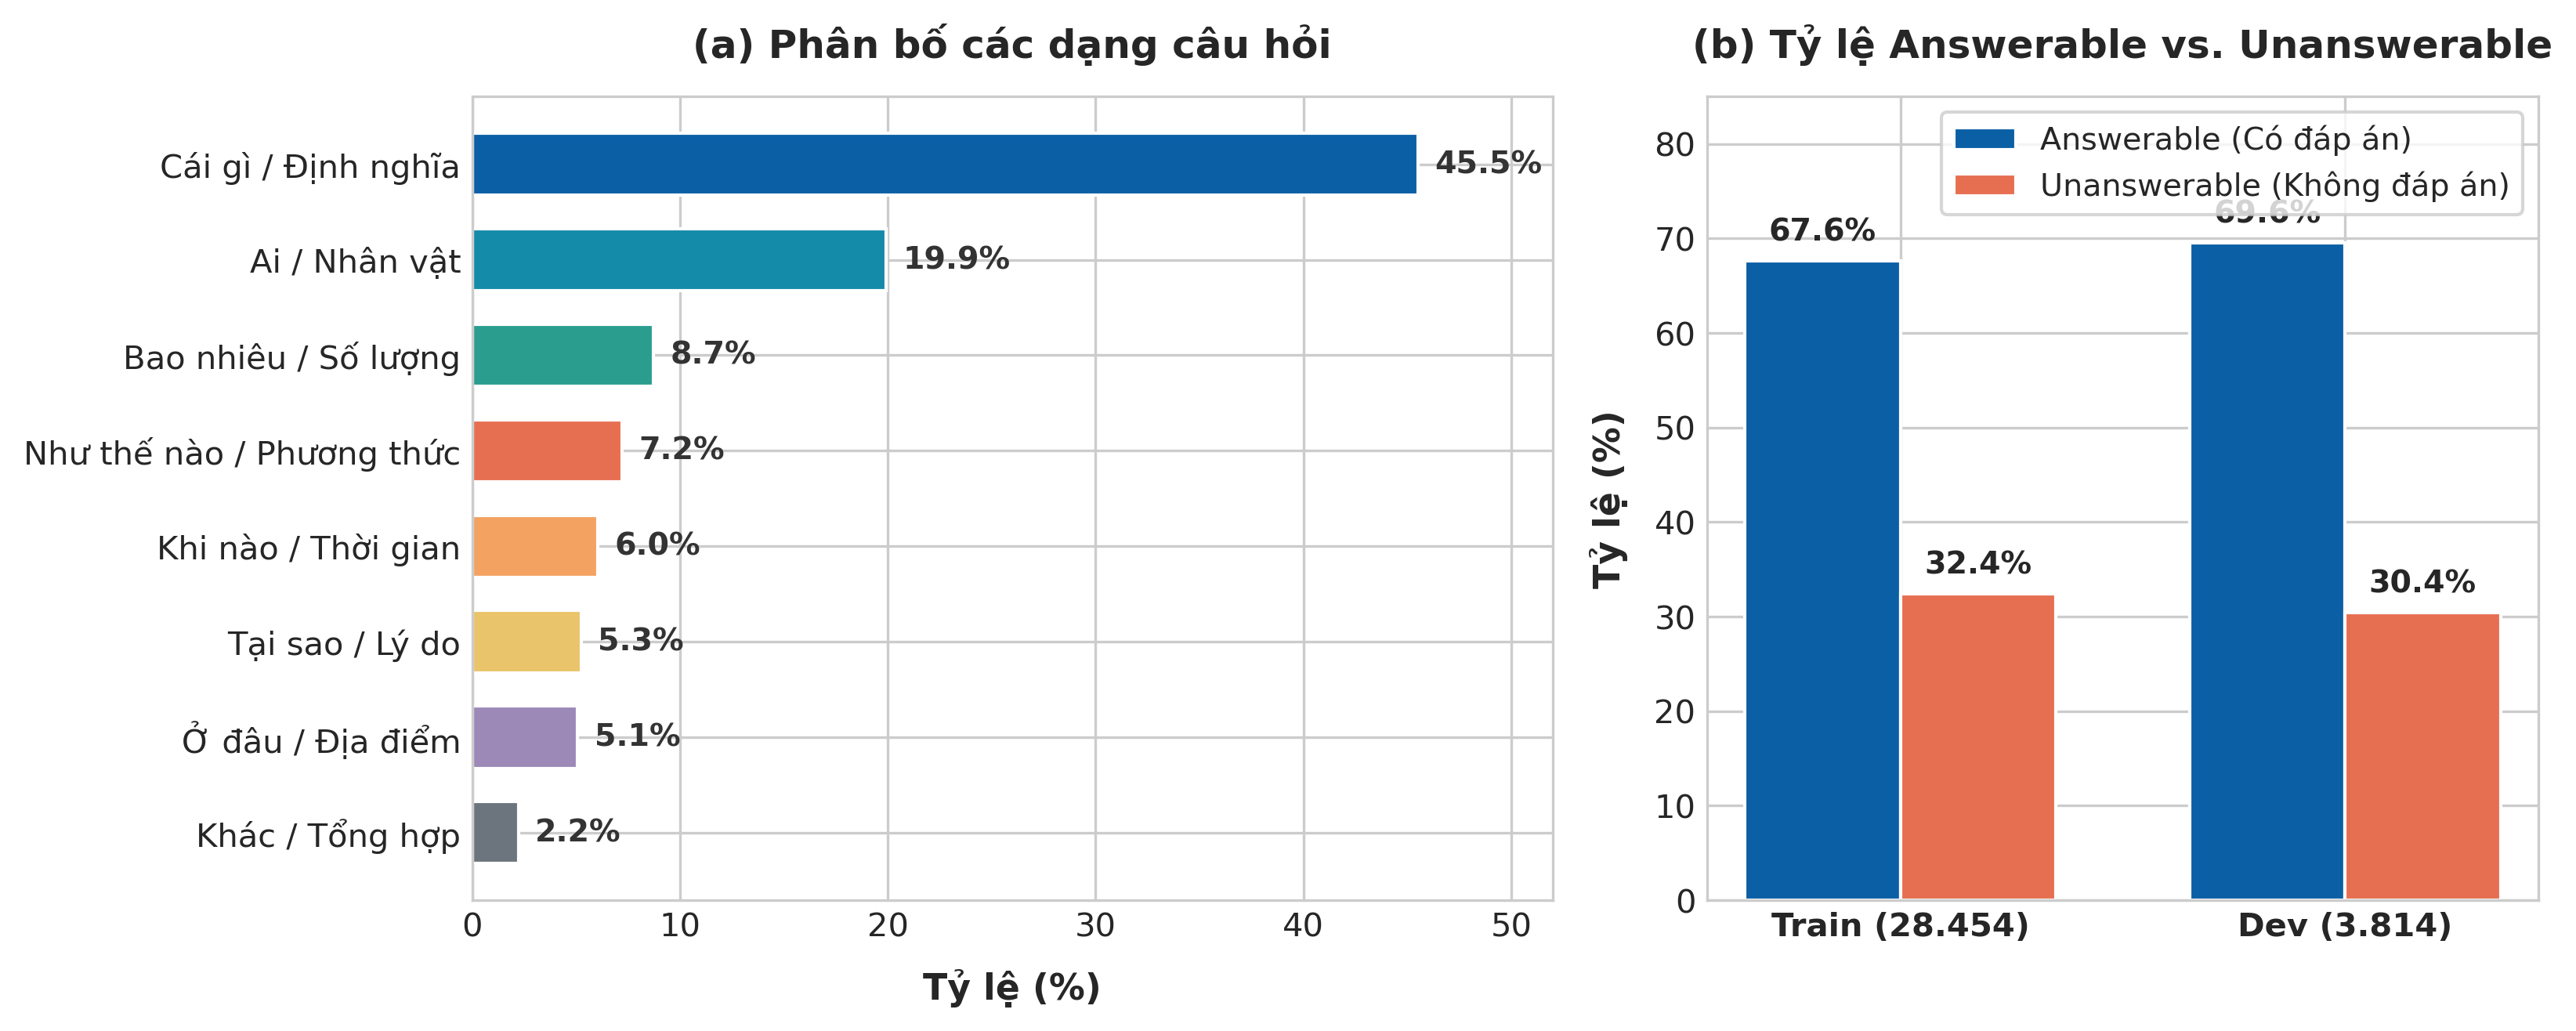
\includegraphics[width=0.95\textwidth]{fig_viquad_dist.png}
\caption{Phân bố dạng câu hỏi và tỷ lệ Answerable/Unanswerable trong bộ dữ liệu}
\label{fig:viquad-dist}
\end{figure}

\subsection{Phân tích Độ dài Văn bản}

Độ dài của văn bản ngữ cảnh, câu hỏi và đáp án ảnh hưởng trực tiếp đến tham số \texttt{max\_seq\_length} của PhoBERT và kích thước cửa sổ chia đoạn. \Cref{tab:length-stats} thể hiện các chỉ số thống kê về số lượng từ (whitespace word count) và số lượng ký tự.

\begin{table}[H]
\centering
\caption{Thống kê độ dài từ và ký tự của các thành phần văn bản}
\label{tab:length-stats}
\begin{tabular}{|L{4.2cm}|C{2.0cm}|C{2.0cm}|C{1.8cm}|C{1.8cm}|C{1.8cm}|}
\hline
\textbf{Thành phần} & \textbf{Trung bình} & \textbf{Trung vị} & \textbf{Nhỏ nhất} & \textbf{Lớn nhất} & \textbf{Độ lệch chuẩn}\\
\hline
Context gốc (Từ) & 177,3 & 159 & 88 & 1.537 & 69,4 \\
\hline
Context gốc (Ký tự) & 820,4 & 732 & 465 & 7.221 & 319,9 \\
\hline
Passage chunked (Từ) & 157,7 & 155 & 33 & 220 & 36,9 \\
\hline
Câu hỏi (Từ) & 14,6 & 14 & 1 & 53 & 5,0 \\
\hline
Span Đáp án (Từ) & 10,0 & 6 & 1 & 150 & 10,6 \\
\hline
\end{tabular}
\end{table}

\Cref{fig:length-dist} mô tả mật độ xác suất (KDE) độ dài từ trước và sau khi chunking. Có thể thấy ngữ cảnh gốc có đuôi kéo dài lên đến 1.537 từ (vượt xa giới hạn 256--384 token của PhoBERT). Kỹ thuật passage chunking đóng gói tối đa 220 từ giúp đưa toàn bộ phân bố độ dài nằm trọn trong ngân sách xử lý của Transformer.

\begin{figure}[H]
\centering
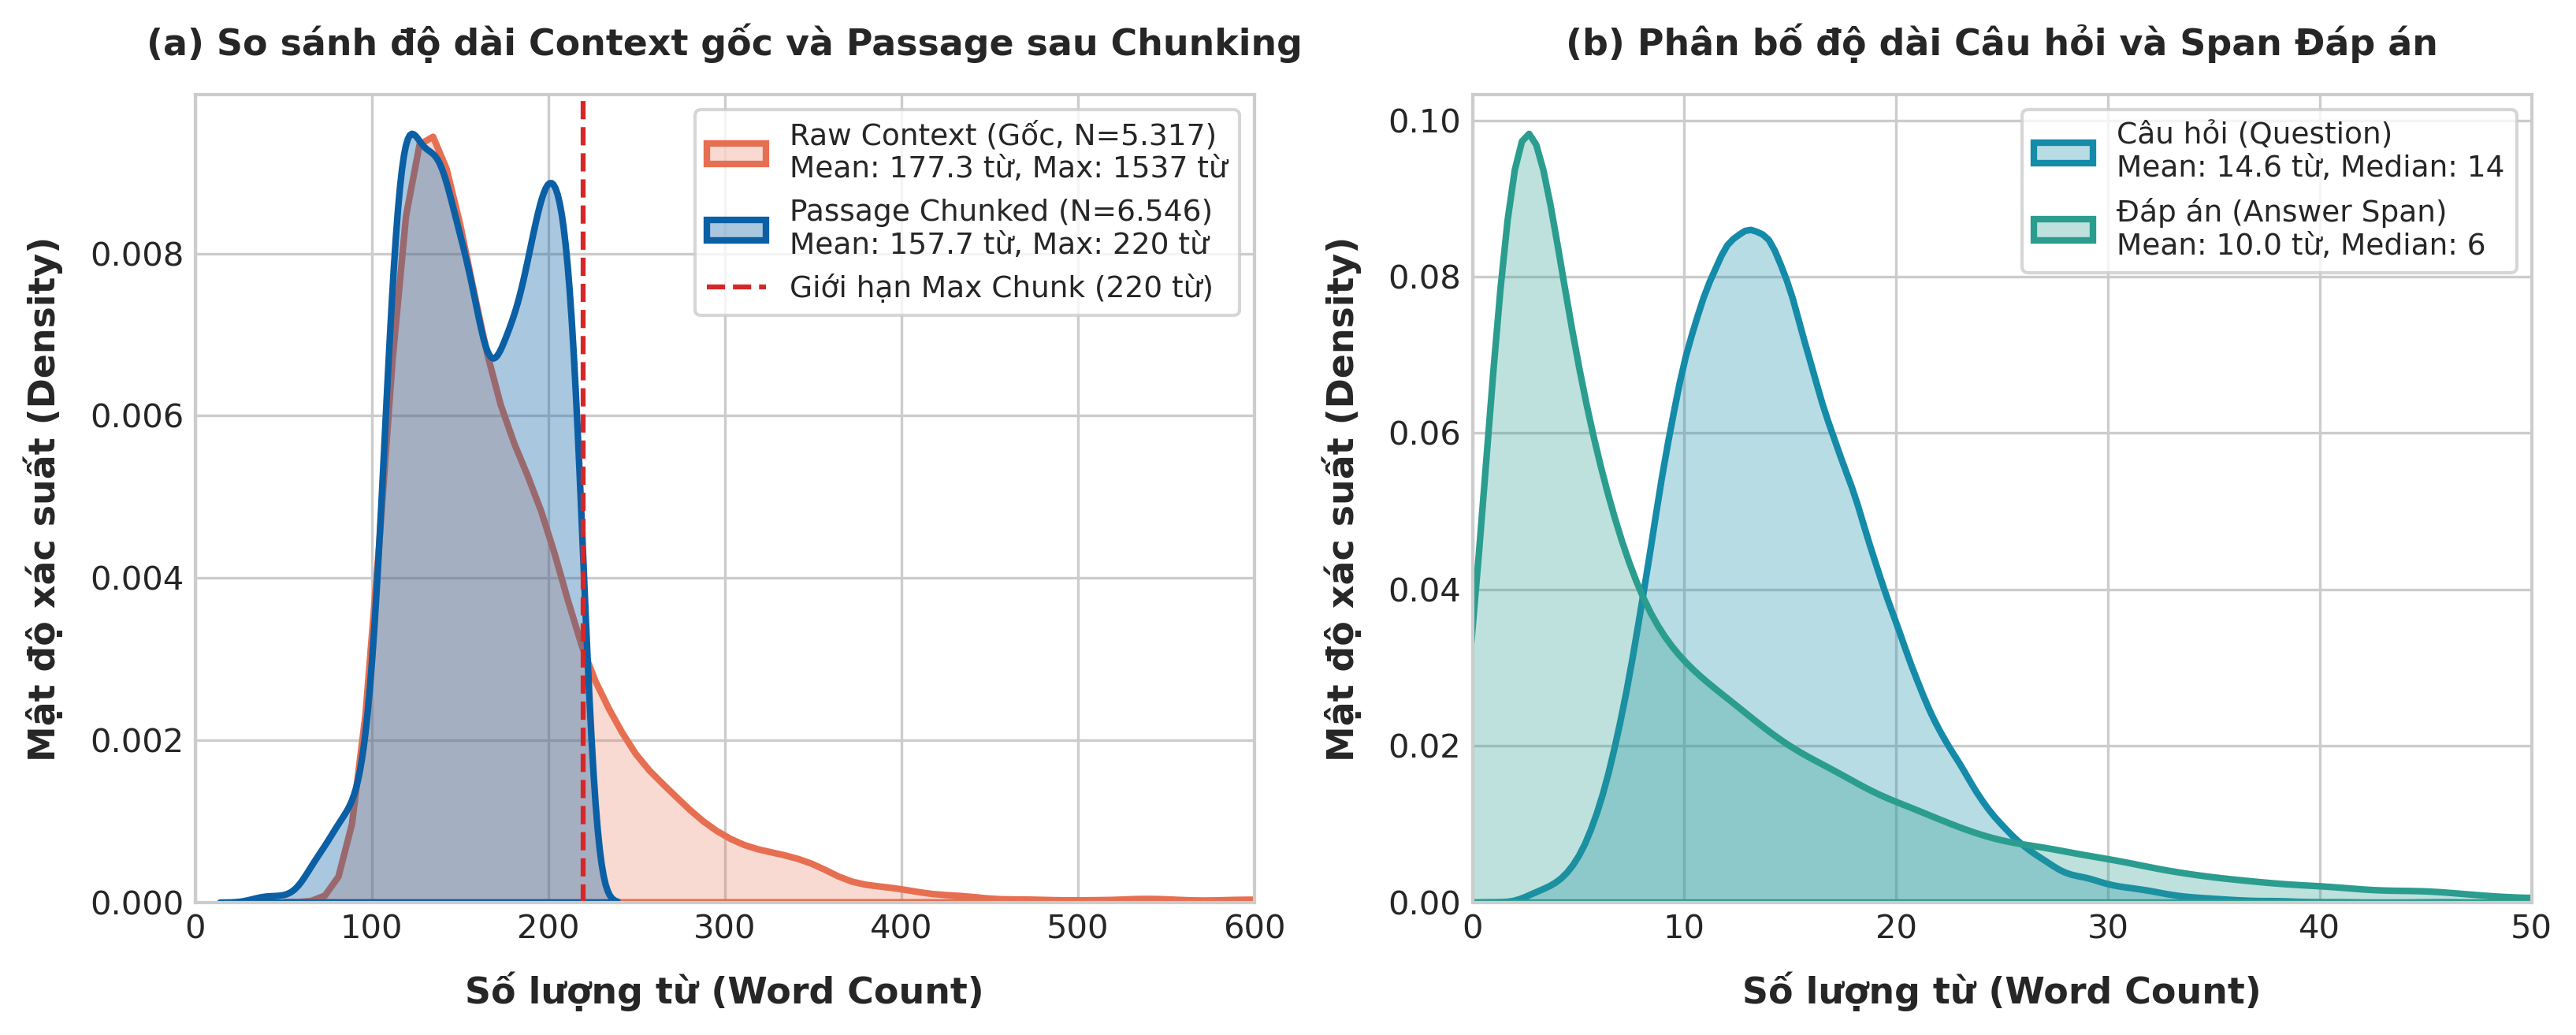
\includegraphics[width=0.95\textwidth]{fig_length_dist.png}
\caption{Mật độ xác suất (KDE) độ dài từ của Context gốc vs. Passage chunked và Câu hỏi vs. Đáp án}
\label{fig:length-dist}
\end{figure}

\section{Đặc thù xử lý ngôn ngữ tiếng Việt và Bài toán Tokenization}
\label{sec:vietnamese-tokenization}

Xử lý tiếng Việt trong hệ thống QA đòi hỏi giải quyết hiện tượng nhập nhằng từ ghép. Khác với tiếng Anh (nơi khoảng trắng phân tách rõ ràng giữa các từ đơn), tiếng Việt sử dụng khoảng trắng cho cả hai mục đích: phân tách âm tiết trong cùng một từ ghép (ví dụ: \textit{``thành phố''}, \textit{``xử lý ngôn ngữ tự nhiên''}) và phân tách giữa các từ khác nhau.

Trong hệ thống VIQA Nexus, dữ liệu được tổ chức dưới hai biểu diễn song song:
\begin{enumerate}
    \item \textbf{Biểu diễn văn bản tự nhiên (Clean Text)}: Giữ nguyên khoảng trắng tự nhiên và các dấu câu chuẩn. Biểu diễn này dùng để hiển thị lên giao diện Web UI, xây dựng chỉ mục SQLite \texttt{docs.db} và tính toán điểm tương đồng thưa TF--IDF / BM25.
    \item \textbf{Biểu diễn tách từ (Segmented Text)}: Đưa qua công cụ tách từ tiếng Việt (\texttt{PyVi}) để nối các âm tiết thuộc cùng một từ ghép bằng dấu gạch dưới (ví dụ: \textit{``thành\_phố''}, \textit{``ngôn\_ngữ\_tự\_nhiên''}). Biểu diễn này bắt buộc phải khớp với cách thức tiền huấn luyện của mô hình \textbf{PhoBERT} \cite{phobert}.
\end{enumerate}

Một nguyên tắc cốt lõi được thiết lập: \textbf{Mọi checkpoint mô hình QA phải sử dụng đúng Fast Tokenizer tương ứng với bước tạo nhãn huấn luyện.} PhoBERT sử dụng giải thuật Byte-Pair Encoding (BPE) phân tách subword trên văn bản đã \texttt{word\_segmented}. Nếu đưa văn bản chưa tách từ vào PhoBERT, các từ ghép sẽ bị tách thành các subword rời rạc sai lệch, làm giảm đáng kể khả năng biểu diễn ngữ nghĩa của mạng Transformer.

\section{Thuật toán Alignment \& Ánh xạ Offset Ký tự}
\label{sec:answer-alignment}

\subsection{Thách thức dịch chuyển Offset ký tự}

Một bài toán kỹ thuật phức tạp phát sinh khi kết hợp PyVi word segmentation với bài toán Extractive QA. Bộ dữ liệu UIT-ViQuAD2.0 gốc lưu trữ vị trí đáp án dưới dạng chỉ số ký tự bắt đầu (\texttt{answer\_start}) trên \textbf{văn bản thô nguyên bản}. Khi áp dụng công cụ tách từ PyVi, khoảng trắng giữa các âm tiết từ ghép bị thay thế bởi dấu gạch dưới (\texttt{\_}). Điều này làm thay đổi tổng độ dài chuỗi và khiến vị trí \texttt{answer\_start} ban đầu bị sai lệch hoàn toàn.

Nếu sử dụng trực tiếp offset cũ để cắt chuỗi trên văn bản segmented, đáp án trích xuất ra sẽ bị lệch từ, mất ký tự đầu/cuối hoặc gán nhãn sai cho mô hình PhoBERT trong quá trình tạo feature huấn luyện.

\subsection{Thuật toán \texttt{find\_char\_span}}

Để khắc phục triệt để rủi ro này, nhóm đã phát triển thuật toán căn chỉnh vị trí \texttt{find\_char\_span}. Thuật toán dựa trên nguyên lý: \textbf{Ký tự chữ cái và chữ số của đoạn đáp án không bao giờ thay đổi, chỉ có dấu khoảng trắng và dấu gạch dưới bị biến đổi do quá trình tách từ.}

Giả sử $C$ là văn bản context (đã segmented hoặc clean) và $A$ là chuỗi đáp án (gold answer text). Thuật toán xây dựng mảng ánh xạ vị trí ký tự hữu hiệu:
\begin{align}
    C_{\text{filtered}} &= \left[\, (c_i, i) \;\middle|\; c_i \in C, \, c_i \notin \{\text{space},\, \text{underscore}\} \,\right] \\
    A_{\text{filtered}} &= \left[\, a_j \;\middle|\; a_j \in A, \, a_j \notin \{\text{space},\, \text{underscore}\} \,\right]
\end{align}
trong đó $i$ là chỉ số ký tự thực tế trong $C$.

Chuỗi lọc $S_C = \sum c_i$ và $S_A = \sum a_j$ được tìm kiếm khớp con:
\begin{equation}
    k = \text{find\_substring}(S_C, S_A)
\end{equation}

Nếu tìm thấy $k \neq -1$, vị trí bắt đầu và kết thúc chính xác trên văn bản $C$ được khôi phục qua chỉ số lưu trữ gốc:
\begin{align}
    \text{start\_char} &= C_{\text{filtered}}[k][1] \\
    \text{end\_char} &= C_{\text{filtered}}[k + |S_A| - 1][1] + 1
\end{align}

\subsection{Đánh giá Hiệu quả Thuật toán}

Thực nghiệm kiểm chứng được tiến hành trên toàn bộ \textbf{19.238 mẫu câu hỏi có đáp án} của tập huấn luyện \texttt{viquad\_train}. Kết quả đối sánh được trình bày trong \Cref{tab:alignment-eval}.

\begin{table}[H]
\centering
\caption{Kết quả đối sánh độ chính xác căn chỉnh đáp án trên tập Train (19.238 mẫu Answerable)}
\label{tab:alignment-eval}
\begin{tabular}{|L{6.0cm}|C{3.0cm}|C{3.0cm}|L{3.0cm}|}
\hline
\textbf{Phương pháp Căn chỉnh} & \textbf{Số mẫu khớp} & \textbf{Tỷ lệ chính xác (\%)} & \textbf{Số mẫu mất nhãn}\\
\hline
Khớp chuỗi con thông thường (\textit{Exact Substring}) & 18.313 & 95,19\% & 925 mẫu lỗi \\
\hline
Thuật toán đề xuất \texttt{find\_char\_span} & \textbf{19.238} & \textbf{100,00\%} & \textbf{0 mẫu lỗi} \\
\hline
\end{tabular}
\end{table}

Kết quả cho thấy nếu chỉ dùng phép so sánh substring thông thường trên segmented text, có tới \textbf{925 mẫu đáp án (4,81\%)} bị thất lạc do khác biệt cách nối từ giữa chuỗi đáp án và ngữ cảnh. Thuật toán \texttt{find\_char\_span} giải quyết triệt để 100\% các trường hợp này, đảm bảo gán nhãn chính xác tuyệt đối \texttt{start\_positions} và \texttt{end\_positions} cho PhoBERT Tokenizer với \texttt{offset\_mapping}.

\Cref{fig:tokenization-pipeline} minh họa tổng thể quy trình tiền xử lý, tách từ và căn chỉnh offset ký tự.

\begin{figure}[H]
\centering
\begin{tikzpicture}[node distance=0.8cm and 0.6cm, auto]
\node[block, text width=2.8cm] (raw) {Raw Text \& Gold Answer\\(UIT-ViQuAD2.0)};
\node[block, right=of raw, text width=2.8cm] (pyvi) {PyVi Word Segmenter\\\texttt{thành\_phố}};
\node[block, right=of pyvi, text width=2.8cm] (strip) {\texttt{find\_char\_span}\\Lọc khoảng trắng/\_};
\node[block, right=of strip, text width=2.8cm] (offset) {PhoBERT Fast Tokenizer\\Offset Mapping};

\node[block, below=of pyvi, text width=2.8cm] (clean) {Clean Text\\(Kho SQLite \texttt{docs.db})};
\node[block, below=of offset, text width=2.8cm] (features) {Training Features\\\texttt{start/end\_positions}};

\draw[flowarrow] (raw) -- (pyvi);
\draw[flowarrow] (pyvi) -- (strip);
\draw[flowarrow] (strip) -- (offset);
\draw[flowarrow] (offset) -- (features);
\draw[flowarrow] (raw) |- (clean);
\end{tikzpicture}
\caption{Quy trình Tách từ, Tokenization và Căn chỉnh Offset Ký tự trong VIQA Nexus}
\label{fig:tokenization-pipeline}
\end{figure}

\section{Sentence Segmentation và Passage Chunking nâng cao}
\label{sec:passage-chunking}

\subsection{Chiến lược chia đoạn văn bản}

Mô hình Reader PhoBERT có giới hạn độ dài đầu vào tối đa là 384 subword token. Trong khi đó, các bài viết Wikipedia gốc có thể dài tới hàng nghìn từ. Nếu cắt đoạn thô (\textit{naive character truncation}), văn bản sẽ bị đứt đoạn giữa câu, vỡ quan hệ chủ ngữ -- vị ngữ và làm mất hoàn toàn bằng chứng trả lời nếu đáp án nằm ở ranh giới cắt.

Nhóm thiết kế giải pháp \textbf{Passage Chunking theo biên câu kết hợp Cửa sổ trượt (Sentence-boundary Overlapping Chunking)} được quản lý tại module \texttt{backend/chunking.py}.

\subsection{Thuật toán Phân đoạn}

Quy trình chunking thực hiện qua 4 bước:
\begin{enumerate}
    \item \textbf{Tách đoạn văn (Paragraph Split)}: Sử dụng biểu thức chính quy \texttt{\detokenize{r"\n\s*\n+"}} để chia ngữ cảnh gốc thành các paragraph độc lập.
    \item \textbf{Tách câu (Sentence Segmentation)}: Áp dụng biểu thức chính quy nhận diện biên câu tiếng Việt:
    \begin{center}
    \texttt{\detokenize{r"(?<=[.!?…])(?:[\"'”’)]*)\s+(?=[A-ZÀ-Ỹ0-9\"'“‘(])"}}
    \end{center}
    giúp tách chính xác các câu mà không bị ngắt sai tại các từ viết tắt phổ biến (như \textit{TP., TS., NXB., v.v.}).
    \item \textbf{Xử lý câu vượt ngưỡng (Oversized Sentence Fallback)}: Nếu một câu đơn vượt quá ngân sách \texttt{max\_tokens} (220 từ), thuật toán tiến hành tách theo dấu chấm phẩy (\texttt{;}), dấu hai chấm (\texttt{:}), dấu phẩy (\texttt{,}). Nếu vẫn dài, câu sẽ được chia theo cửa sổ từ.
    \item \textbf{Đóng gói Cửa sổ trượt (Sentence Overlapping Packing)}: Gộp các câu liên tiếp cho đến khi tổng số từ đạt tối đa 220 từ. Khi chuyển sang chunk tiếp theo, 2 câu cuối cùng của chunk trước được giữ lại làm gối đầu (\textit{overlap 2 sentences}).
\end{enumerate}

\subsection{Phân tích Hiệu quả Kỹ thuật}

Chiến lược gối đầu 2 câu đem lại 3 ưu thế quan trọng:
\begin{itemize}
    \item \textbf{Loại bỏ rủi ro biên}: Đảm bảo đáp án không bao giờ bị cắt đôi do nằm đúng vị trí ranh giới giữa hai passage.
    \item \textbf{Bảo toàn ngữ cảnh giải nghĩa}: Giúp Reader luôn đọc được câu dẫn nhập ngay trước đáp án để hiểu đại từ thay thế (như \textit{``Ông'', ``Bà'', ``Thành phố này''}).
    \item \textbf{Tối ưu quy mô kho tìm kiếm}: Quy mô kho tri thức tăng từ 5.317 document gốc lên 6.546 passage. Độ dài trung bình của mỗi passage đạt 157,7 từ (độ lệch chuẩn 36,9 từ), hoàn toàn vừa vặn trong cửa sổ suy luận của PhoBERT, giúp giảm thiểu chi phí trích xuất câu và tăng đáng kể chỉ số Recall@k của tầng Retriever.
\end{itemize}

\section{Xây dựng Kho tri thức (Corpus \& SQLite \texttt{docs.db})}
\label{sec:corpus-construction}

Toàn bộ văn bản sau khi chuẩn hóa được đưa vào kho lưu trữ có cấu trúc phục vụ thời gian thực (runtime).

\begin{figure}[H]
\centering
\begin{tikzpicture}[node distance=0.85cm and 0.7cm]
\node[block] (raw) {Raw UIT-ViQuAD2.0\\Parquet};
\node[block,right=of raw] (clean) {Chuẩn hóa schema\\và Unicode};
\node[block,right=of clean] (split) {Clean / Segmented\\datasets};
\node[block,below=of clean] (corpus) {Hợp nhất context\\5.317 documents};
\node[block,left=of corpus] (db) {SQLite\\\texttt{docs.db}};
\node[block,right=of corpus] (passage) {Runtime chunking\\6.544 passages};
\draw[flowarrow] (raw) -- (clean);
\draw[flowarrow] (clean) -- (split);
\draw[flowarrow] (clean) -- (corpus);
\draw[flowarrow] (corpus) -- (db);
\draw[flowarrow] (corpus) -- (passage);
\end{tikzpicture}
\caption{Luồng chuẩn bị dữ liệu và xây dựng cơ sở dữ liệu kho tri thức VIQA Nexus}
\label{fig:data-pipeline}
\end{figure}

Dữ liệu được lưu trữ dưới hai định dạng chuyên biệt:
\begin{itemize}
    \item \textbf{Tệp Parquet chuẩn hóa} (\texttt{corpus\_clean.parquet}): Lưu trữ toàn bộ 5.317 văn bản ngữ cảnh duy nhất cùng định danh \texttt{id}, \texttt{title}, \texttt{text}.
    \item \textbf{Cơ sở dữ liệu SQLite} (\texttt{data/processed/docs.db}): Lưu trữ bảng \texttt{documents} phục vụ truy vấn HTTP API thời gian thực. Khi dịch vụ backend khởi tạo, hệ thống đọc dữ liệu từ SQLite, thực hiện chunking tự động và nạp chỉ mục passage lên bộ nhớ RAM để đảm bảo tốc độ phản hồi tính bằng mili-giây.
\end{itemize}

Mỗi passage đầu ra mang đầy đủ siêu dữ liệu truy vết: \texttt{document\_id}, \texttt{passage\_id} (dạng \texttt{DOC0001\_P0001}), \texttt{title}, \texttt{paragraph\_id}, chỉ số câu bắt đầu/kết thúc và chuỗi văn bản \texttt{text}. Cấu trúc này cho phép giao diện Web UI hiển thị chính xác trích dẫn nguồn bằng chứng cho người dùng cuối.

\chapter{Thiết kế hệ thống hỏi đáp tiếng Việt}
\label{chap:design}

\section{Kiến trúc tổng thể}
VIQA Nexus được thiết kế theo kiến trúc open-domain extractive QA hai tầng. Tầng đầu tiên
thu hẹp corpus thành một tập nhỏ passage liên quan; tầng thứ hai đọc từng passage để dự đoán
span trả lời. Sau đó một bước hợp nhất điểm lựa chọn câu trả lời cuối cùng. Cách phân rã này
giúp hệ thống xử lý corpus lớn hơn giới hạn ngữ cảnh của Transformer và cho phép đánh giá
riêng lỗi Retriever với lỗi Reader.

\begin{figure}[H]
\centering
\begin{tikzpicture}[node distance=0.55cm and 0.28cm]
\node[smallblock] (q) {Câu hỏi};
\node[smallblock,right=of q] (ret) {Retriever};
\node[smallblock,right=of ret] (topk) {Top-$k$\\passages};
\node[smallblock,right=of topk] (reader) {PhoBERT\\Reader};
\node[smallblock,right=of reader] (rank) {Reranking};
\node[smallblock,right=of rank] (answer) {Câu trả lời\\và nguồn};
\draw[flowarrow] (q) -- (ret);
\draw[flowarrow] (ret) -- (topk);
\draw[flowarrow] (topk) -- (reader);
\draw[flowarrow] (reader) -- (rank);
\draw[flowarrow] (rank) -- (answer);
\end{tikzpicture}
\caption{Kiến trúc xử lý câu hỏi của VIQA Nexus}
\label{fig:qa-architecture}
\end{figure}

Đầu vào của pipeline là chuỗi câu hỏi tiếng Việt và ba tham số: phương pháp Retriever,
Reader, và $k$. Đầu ra không chỉ là answer text mà còn gồm confidence, thời gian, phương
pháp trích xuất, document ID, passage ID và danh sách passage nguồn. Thiết kế này hỗ trợ
truy vết quyết định của hệ thống thay vì chỉ hiển thị một chuỗi không có căn cứ.

\section{Retriever TF--IDF}
Baseline TF--IDF biểu diễn câu hỏi và passage trong cùng không gian sparse. Chỉ mục lưu
vocabulary, IDF và ma trận passage; khi truy vấn, hệ thống vector hóa câu hỏi rồi tính cosine
similarity. Đây là baseline gần với hướng tiếp cận của DrQA, dễ kiểm tra và có tốc độ truy vấn
cao trên corpus hiện tại. Hạn chế chính là phụ thuộc trùng khớp từ bề mặt: hai biểu thức đồng
nghĩa nhưng dùng từ khác nhau có thể có similarity thấp.

Trong API sản phẩm, TF--IDF là một trong hai Retriever hoạt động thật. Chỉ mục được tạo một
lần và tái sử dụng giữa các request. Kết quả trả về gồm định danh passage, nội dung và raw
retrieval score; score sau đó được chuẩn hóa trên tập ứng viên trước khi hợp nhất với Reader.

\section{Retriever BM25}
BM25 dùng tần suất từ có saturation và chuẩn hóa theo độ dài passage. Cấu hình cụ thể của
$k_1$ và $b$ được quản lý tại module retrieval; báo cáo không tuyên bố đây là bộ tham số tối
ưu vì chưa có thí nghiệm grid search độc lập. So với TF--IDF, BM25 thường xử lý tốt hơn từ
khóa xuất hiện nhiều lần và passage có độ dài khác nhau. Kết quả thực nghiệm ở
\cref{chap:experiments} cho thấy BM25 đứng đầu cả Recall và MRR trên tập test hiện có, đổi
lại QPS thấp hơn đáng kể.

BM25 là Retriever thứ hai đã được nối thật vào endpoint hỏi đáp. Nó cũng được dùng trong ví
dụ request/response và trong chế độ so sánh Retriever của giao diện.

\section{Dense Retrieval và FAISS}
Dense Retriever dùng Sentence Transformers để ánh xạ câu hỏi và passage thành embedding
dày, sau đó tìm kiếm lân cận gần bằng FAISS. Module này đã được cài đặt và benchmark offline.
Ưu điểm kỳ vọng là truy hồi theo ngữ nghĩa khi câu hỏi không lặp đúng từ khóa của passage.
Tuy nhiên, checkpoint tổng quát chưa được fine-tune theo cặp question--positive passage của
UIT-ViQuAD2.0, nên kết quả hiện tại thấp hơn hai phương pháp sparse.

Dense Retrieval chưa được nối vào API sản phẩm. Vì vậy nhãn Dense từng xuất hiện trong giao
diện không được xem là bằng chứng rằng backend đã chạy Dense. Báo cáo tách rõ ``đã có module
và benchmark offline'' khỏi ``đã tích hợp end-to-end'' để tránh đánh đồng mức hoàn thiện.

\section{Pyserini Retriever}
Pyserini cung cấp giao diện Python cho Lucene và hỗ trợ cả sparse lẫn dense retrieval
\cite{pyserini}. Project có implementation Pyserini thật thay vì một lớp giả lập. Tuy vậy,
repo chưa lưu đầy đủ Lucene index, chưa có benchmark chính thức tương ứng trong
\texttt{results/}, và chưa kết nối Pyserini vào endpoint sản phẩm. Do đó Pyserini được xếp vào
nhóm thử nghiệm kỹ thuật cần hoàn thiện, không đặt ngang hàng với một thuật toán như BM25.

\section{Lựa chọn Top-\texorpdfstring{$k$}{k} passage}
Giá trị mặc định mà client gửi là $k=5$. Backend có thể lấy tối đa 10 ứng viên nội bộ trước
khi Reader và reranker lựa chọn. Tăng $k$ thường cải thiện khả năng passage đúng xuất hiện,
nhưng thời gian Reader tăng gần tuyến tính theo số cửa sổ cần suy luận và số distractor cũng
tăng. Cấu hình 5/10 là cân bằng thực dụng hiện tại; chưa có ablation đủ để gọi là tối ưu.

Mỗi ứng viên được chuẩn hóa retrieval score bằng min--max trong cùng request:
\begin{equation}
\widehat{s}_{r,i}=\frac{s_{r,i}-\min_j s_{r,j}}
{\max_j s_{r,j}-\min_j s_{r,j}+\epsilon}.
\label{eq:retrieval-normalization}
\end{equation}
Chuẩn hóa này giúp kết hợp score từ các Retriever có miền giá trị khác nhau, nhưng khiến
score mang tính tương đối theo tập ứng viên, không phải xác suất hiệu chỉnh toàn cục.

\section{PhoBERT Reader}
Reader sản phẩm dùng checkpoint \texttt{models/reader/vinai\_phobert-base-v2}, được nạp qua
\texttt{AutoModelForQuestionAnswering} và hiện thực bởi
\texttt{RobertaForQuestionAnswering} của thư viện Transformers \cite{transformers}.
Checkpoint được fine-tune từ PhoBERT-base-v2 trên bản
segmented của UIT-ViQuAD2.0 trong 5 epoch; artifact được ghi nhận ở bước 4.500 với tệp trọng
số 537.660.768 byte (xấp xỉ 513 MiB). Những thông tin này mô tả artifact trong repo, không
thay thế cho log huấn luyện đầy đủ hoặc thí nghiệm lặp nhiều seed.

\begin{figure}[H]
\centering
\begin{tikzpicture}[node distance=0.70cm and 0.38cm]
\node[smallblock] (input) {Question + Context};
\node[smallblock,right=of input] (tok) {Fast tokenizer\\offset mapping};
\node[smallblock,right=of tok] (enc) {PhoBERT\\Transformer encoder};
\node[smallblock,right=of enc] (head) {QA head};
\node[smallblock,above right=0.22cm and 0.55cm of head] (start) {Start logits};
\node[smallblock,below right=0.22cm and 0.55cm of head] (end) {End logits};
\node[smallblock,right=3.0cm of head] (span) {Answer span};
\draw[flowarrow] (input) -- (tok);
\draw[flowarrow] (tok) -- (enc);
\draw[flowarrow] (enc) -- (head);
\draw[flowarrow] (head) -- (start);
\draw[flowarrow] (head) -- (end);
\draw[flowarrow] (start) -- (span);
\draw[flowarrow] (end) -- (span);
\end{tikzpicture}
\caption{Luồng dự đoán span của PhoBERT Reader}
\label{fig:reader-flow}
\end{figure}

Chỉ PhoBERT được chạy thật trong pipeline sản phẩm. XLM-R mới xuất hiện ở notebook thử
nghiệm và không có production checkpoint; viBERT chưa được triển khai. Vì thế các lựa chọn
Reader không hoạt động thật phải bị loại hoặc khóa trên UI cho đến khi backend cung cấp.

\section{Trích xuất answer span}
Tokenizer nhanh tạo \texttt{offset\_mapping} để ánh xạ token trở lại vị trí ký tự trong context.
Với context dài, sliding window chia input thành nhiều feature có overlap. Model trả về
\texttt{start\_logits} và \texttt{end\_logits}; hệ thống duyệt các cặp vị trí hợp lệ, loại span nằm
ngoài context, span có end trước start và span vượt độ dài tối đa. Cặp tốt nhất được chuyển
ngược qua offset để lấy đúng substring của passage.

Batch inference được dùng cho nhiều passage/cửa sổ nhằm giảm overhead gọi model. Tuy vậy,
môi trường hiện tại dùng PyTorch CPU, nên số candidate và độ dài sequence vẫn ảnh hưởng lớn
đến latency. Một span hợp lệ về mặt chỉ số cũng chưa chắc là câu trả lời tốt về ngữ nghĩa;
đó là lý do cần threshold, fallback có kiểm soát và đánh giá answerable riêng.

\section{Xử lý câu hỏi không có đáp án}
Reader dành vị trí đặc biệt cho no-answer và so sánh score null với score span. Ngưỡng
no-answer hiện tại là 0,30. Nếu bằng chứng thấp, hệ thống có thể trả về thông báo không tìm
thấy câu trả lời đủ tin cậy thay vì buộc chọn một span. Ngưỡng này là cấu hình vận hành, chưa
được chứng minh tối ưu bằng precision--recall curve trên dev.

Kết quả oracle cho thấy mô hình thiên lệch mạnh về no-answer: EM trên câu không có đáp án
cao nhưng EM/F1 trên câu có đáp án rất thấp. Vì vậy tăng threshold đơn thuần có thể thay đổi
tỷ lệ từ chối nhưng không giải quyết gốc rễ. Cần kiểm tra cân bằng dữ liệu, alignment span,
loss, checkpoint và calibration như đề xuất ở \cref{chap:conclusion}.

\section{Fallback answer extraction}
Khi neural Reader không tạo span đủ tin cậy hoặc phát sinh điều kiện bất thường, pipeline có
fallback dựa trên câu trong passage. Fallback ưu tiên câu có liên hệ từ khóa với câu hỏi và
trả về câu hoàn chỉnh hơn một mẩu entity bị cắt. Đây là cơ chế tăng khả năng demo và giúp câu
trả lời ``ai'' có ngữ cảnh giải thích; nó không phải bằng chứng Reader neural đã dự đoán đúng.
Response API luôn ghi trường \texttt{method}, nhờ đó có thể phân biệt kết quả \texttt{neural}
với \texttt{fallback} khi đánh giá.

Fallback cũng có rủi ro đưa thêm mệnh đề không cần thiết hoặc chọn câu chứa entity nhưng
không định nghĩa entity. Do vậy chất lượng của nó phải được đo riêng và không trộn vào chỉ số
Reader oracle.

\section{Reranking kết hợp Retriever và Reader}
Với neural Reader, tín hiệu đọc được tính từ confidence và normalized margin:
\begin{equation}
s_{\text{reader},i}=0{,}75c_i+0{,}25\widehat{m}_i,
\label{eq:reader-signal}
\end{equation}
trong đó $c_i$ là confidence và $\widehat{m}_i$ là margin giữa span và null score sau chuẩn
hóa. Với fallback, $s_{\text{reader},i}=c_i$. Điểm cuối cùng là:
\begin{equation}
s_{\text{final},i}=0{,}15\widehat{s}_{r,i}+0{,}85s_{\text{reader},i}.
\label{eq:final-score}
\end{equation}

Các trọng số 0,15; 0,75; 0,25 và 0,85 là cấu hình hiện tại của phần mềm, không được trình bày
như hằng số tối ưu phổ quát. Chúng cần được tuning trên dev bằng metric end-to-end, sau đó
khóa lại trước khi đánh giá test. Việc dùng Reader signal lớn giúp passage có answer span rõ
vượt lên, nhưng một Reader lệch no-answer hoặc confidence chưa calibration có thể làm
reranking sai mạnh hơn.

\section{Lựa chọn và đóng gói câu trả lời cuối}
Ứng viên có $s_{\text{final}}$ cao nhất và vượt điều kiện tin cậy được chọn. Backend đóng gói
answer, confidence, scores, source và top passages thành JSON. Câu trả lời được trim khoảng
trắng nhưng không tự sinh thêm tri thức ngoài passage. Khi method là fallback, answer có thể
là một câu đầy đủ; khi method là neural, answer thường là span ngắn. Frontend phải trình bày
cả answer và source để người dùng tự kiểm tra ngữ cảnh.

\chapter{Cài đặt hệ thống}
\label{chap:implementation}

\section{Kiến trúc phần mềm}
Project tách frontend React khỏi backend Python nhưng phân phối trong cùng repository. Trình
duyệt gửi JSON qua HTTP; server điều phối Retriever và Reader rồi trả response có cấu trúc.
Backend hiện dùng \texttt{ThreadingHTTPServer} của thư viện chuẩn, không phải FastAPI. Điều
này đủ cho demo cục bộ, nhưng chưa cung cấp validation schema, OpenAPI hay lifecycle quản lý
model như một framework web chuyên dụng.

\begin{figure}[H]
\centering
\begin{tikzpicture}[node distance=1.0cm and 1.1cm]
\node[block] (react) {React + TypeScript\\Vite frontend};
\node[block,right=of react] (http) {Python\\ThreadingHTTPServer};
\node[block,above right=0.40cm and 1.15cm of http] (ret) {TF--IDF / BM25\\Retriever};
\node[block,below right=0.40cm and 1.15cm of http] (reader) {PhoBERT\\Reader + fallback};
\draw[flowarrow,<->] (react) -- node[above,font=\small]{JSON/HTTP} (http);
\draw[flowarrow,<->] (http) -- (ret);
\draw[flowarrow,<->] (http) -- (reader);
\end{tikzpicture}
\caption{Kiến trúc phần mềm đang được triển khai}
\label{fig:software-architecture}
\end{figure}

\begin{table}[H]
\centering
\small
\caption{Các công nghệ chính của hệ thống}
\label{tab:software-stack}
\begin{tabularx}{\textwidth}{|L{0.18\textwidth}|L{0.25\textwidth}|Y|Y|}
\hline
Lớp & Công nghệ & Vai trò & Trạng thái \\
\hline
Frontend & React 18, TypeScript, Vite & UI hỏi đáp và điều phối trạng thái & Hoạt động \\
\hline
3D & Three.js, React Three Fiber, Drei, \texttt{@pixiv/\allowbreak three-vrm} & Render Mari VRM & Hoạt động \\
\hline
Backend & Python \texttt{ThreadingHTTP\allowbreak Server} & Endpoint hỏi đáp và file service & Hoạt động \\
\hline
Sparse IR & scikit-learn / BM25 modules & TF--IDF và BM25 & Tích hợp API \\
\hline
Dense IR & Sentence Transformers, FAISS & Embedding và vector search & Offline \\
\hline
Reader & PyTorch, Transformers, PhoBERT & Start/end span prediction & Tích hợp API \\
\hline
Dữ liệu & Parquet, SQLite & QA splits và document store & Hoạt động \\
\hline
Đánh giá & Python scripts, JSON/CSV results & Retrieval/Reader benchmark & Một phần \\
\hline
\end{tabularx}
\end{table}

\section{Cấu trúc mã nguồn}
Mã nguồn của hệ thống được lưu tại:
\begin{center}
\url{https://github.com/duong158/QA_system}
\end{center}

Các vùng trách nhiệm chính của repository được tổ chức như sau:
\begin{Verbatim}[fontsize=\scriptsize,frame=single]
QA_system/
|-- src/                         React/TypeScript frontend
|-- backend/
|   |-- viqa_api.py              HTTP API and orchestration
|   `-- chunking.py              Runtime passage chunking
|-- retrieval/                   TF-IDF, BM25, Dense, Pyserini
|-- reader/                      Training and inference utilities
|-- data/                        QA splits, corpus and indexes
|-- models/reader/               Production PhoBERT QA checkpoint
|-- results/                     Stored benchmark artifacts
|-- notebooks/                   Exploration and training notebooks
|-- tests/                       Automated checks
`-- evaluate_qa.py               QA evaluation entry point
\end{Verbatim}

Sơ đồ trên chỉ mô tả nhóm thư mục quan trọng cho báo cáo; các tệp build, cache và dependency
không được liệt kê. Phân tách này cho phép Người 1 cải tiến retrieval, Người 2 huấn luyện
Reader, Người 3 chuẩn hóa dữ liệu và Người 4 tích hợp mà giảm xung đột mã nguồn.

\section{Backend API}
Endpoint chính nhận request dạng sau:
\begin{Verbatim}[fontsize=\scriptsize,frame=single]
POST /api/ask
Content-Type: application/json

{
  "question": "Phạm Văn Đồng là ai?",
  "retriever": "bm25",
  "reader": "phobert",
  "top_k": 5
}
\end{Verbatim}

Backend kiểm tra câu hỏi, chọn một Retriever đã hỗ trợ, lấy candidates, chạy Reader theo
batch và trả answer cùng bằng chứng. Một response chạy thật đã quan sát có answer là một câu
đầy đủ về Phạm Văn Đồng, confidence 0,70, passage \texttt{doc\_00001\_P001}, latency 7.342 ms,
method \texttt{fallback} và final score 0,745. Đây là một mẫu quan sát, không phải latency
trung bình và không được dùng thay benchmark end-to-end.

\section{Cài đặt các module truy hồi}
Thư mục \texttt{retrieval/} chứa interface chung cho document/passage result và các hiện thực
TF--IDF, BM25, Dense, Pyserini. \texttt{build\_index.py} tạo index cần thiết;
\texttt{run\_benchmark.py} điều phối thực nghiệm; \texttt{retrieval/evaluate.py} tính Recall@k
và MRR. Notebook \texttt{notebooks/retrieval\_bm25\_best.ipynb} lưu quá trình khảo sát BM25.
Artifacts trong \texttt{results/} được dùng làm nguồn số liệu cho \cref{tab:retriever-results}.

API chỉ ánh xạ hai giá trị hợp lệ \texttt{tfidf} và \texttt{bm25}. Việc giới hạn này làm trạng
thái sản phẩm nhất quán với backend, đồng thời vẫn giữ Dense/Pyserini để phát triển tiếp.

\section{Cài đặt Reader}
Reader nạp tokenizer nhanh và QA checkpoint một lần khi dịch vụ khởi tạo. Các top passage
được tokenize theo batch với truncation, stride và offset mapping. Vòng chọn span dùng logits,
mask token context và giới hạn độ dài đáp án. Response ghi cả confidence, margin và method để
reranker cũng như script đánh giá có thể kiểm tra.

Checkpoint hơn 500 MiB làm tăng đáng kể thời gian clone và khởi động. Trong Git, artifact cần
được quản lý bằng Git LFS hoặc script tải có checksum; không nên commit như blob Git thông
thường. Báo cáo chỉ ghi nhận checkpoint local đã dùng, không giả định mọi máy pull repo đều
tự động có model nếu cơ chế phân phối chưa được xác minh.

\section{Frontend hỏi đáp}
Frontend React quản lý vòng đời một lượt hỏi: nhập câu hỏi, retrieving, reading, composing và
hoàn tất. Answer panel hiển thị câu trả lời, confidence, source passage, Retriever/Reader và
latency. Các passage top-$k$ có nút xem nguồn; thao tác phải mở hoặc cuộn đến passage tương
ứng thay vì là nút trang trí.

\begin{figure}[H]
\centering
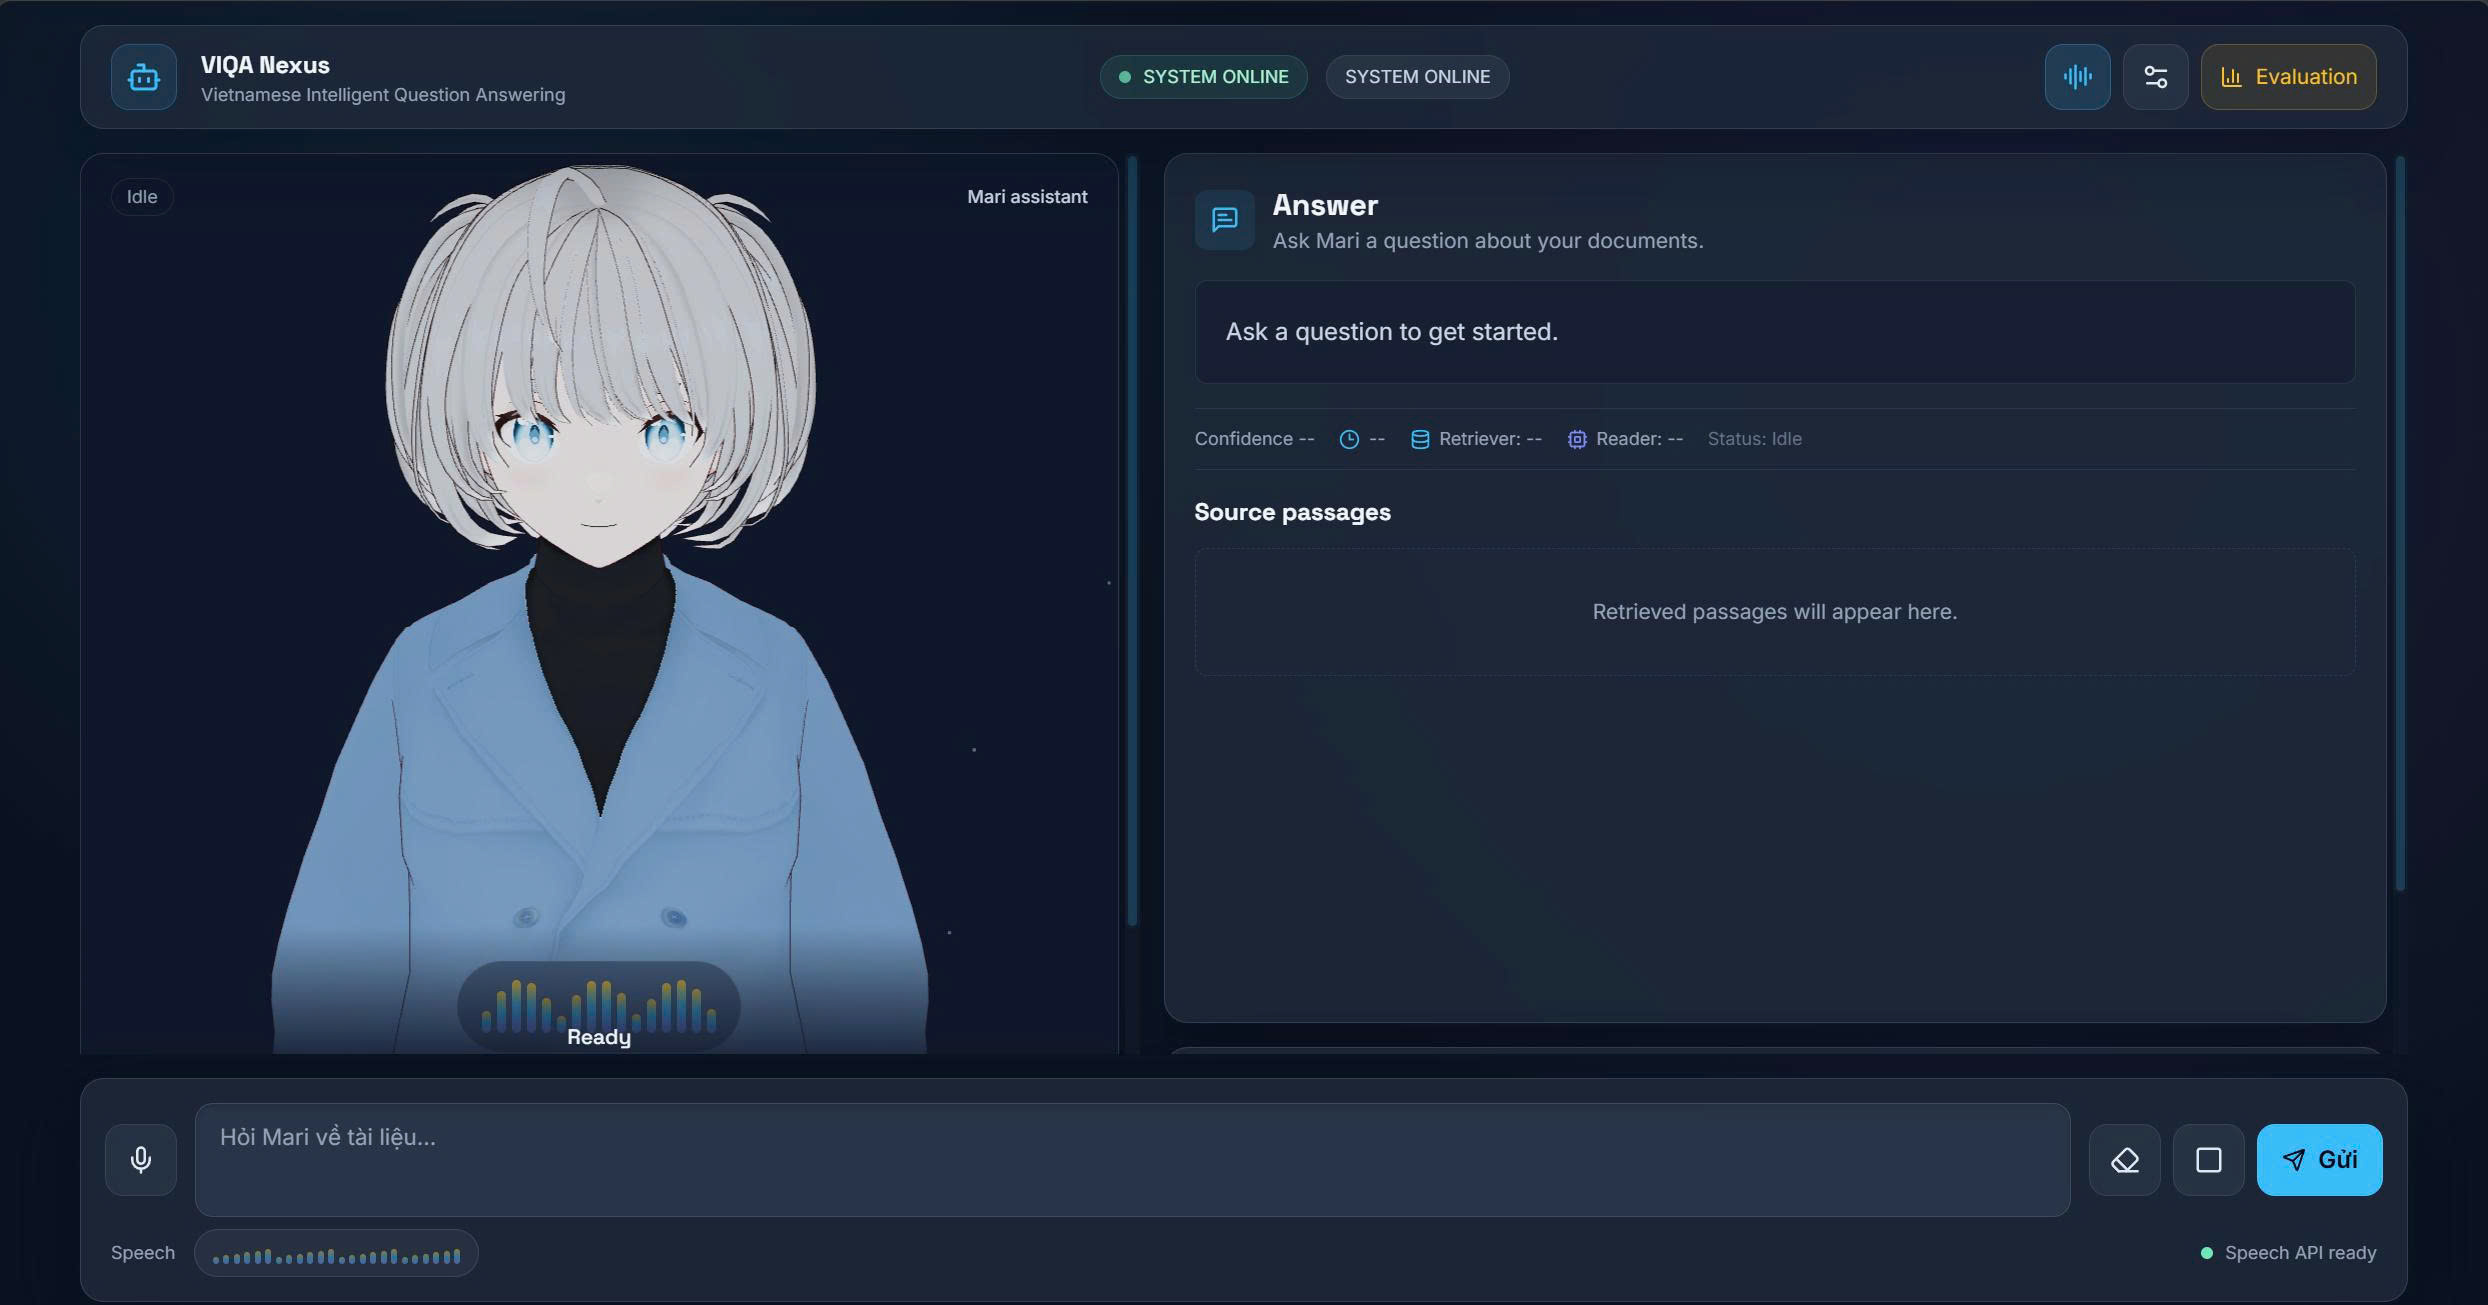
\includegraphics[width=0.95\textwidth]{UI_VIQA_Nexus.jpg}
\caption{Giao diện chính của hệ thống VIQA Nexus}
\label{fig:main-ui}
\end{figure}

\begin{figure}[H]
\centering
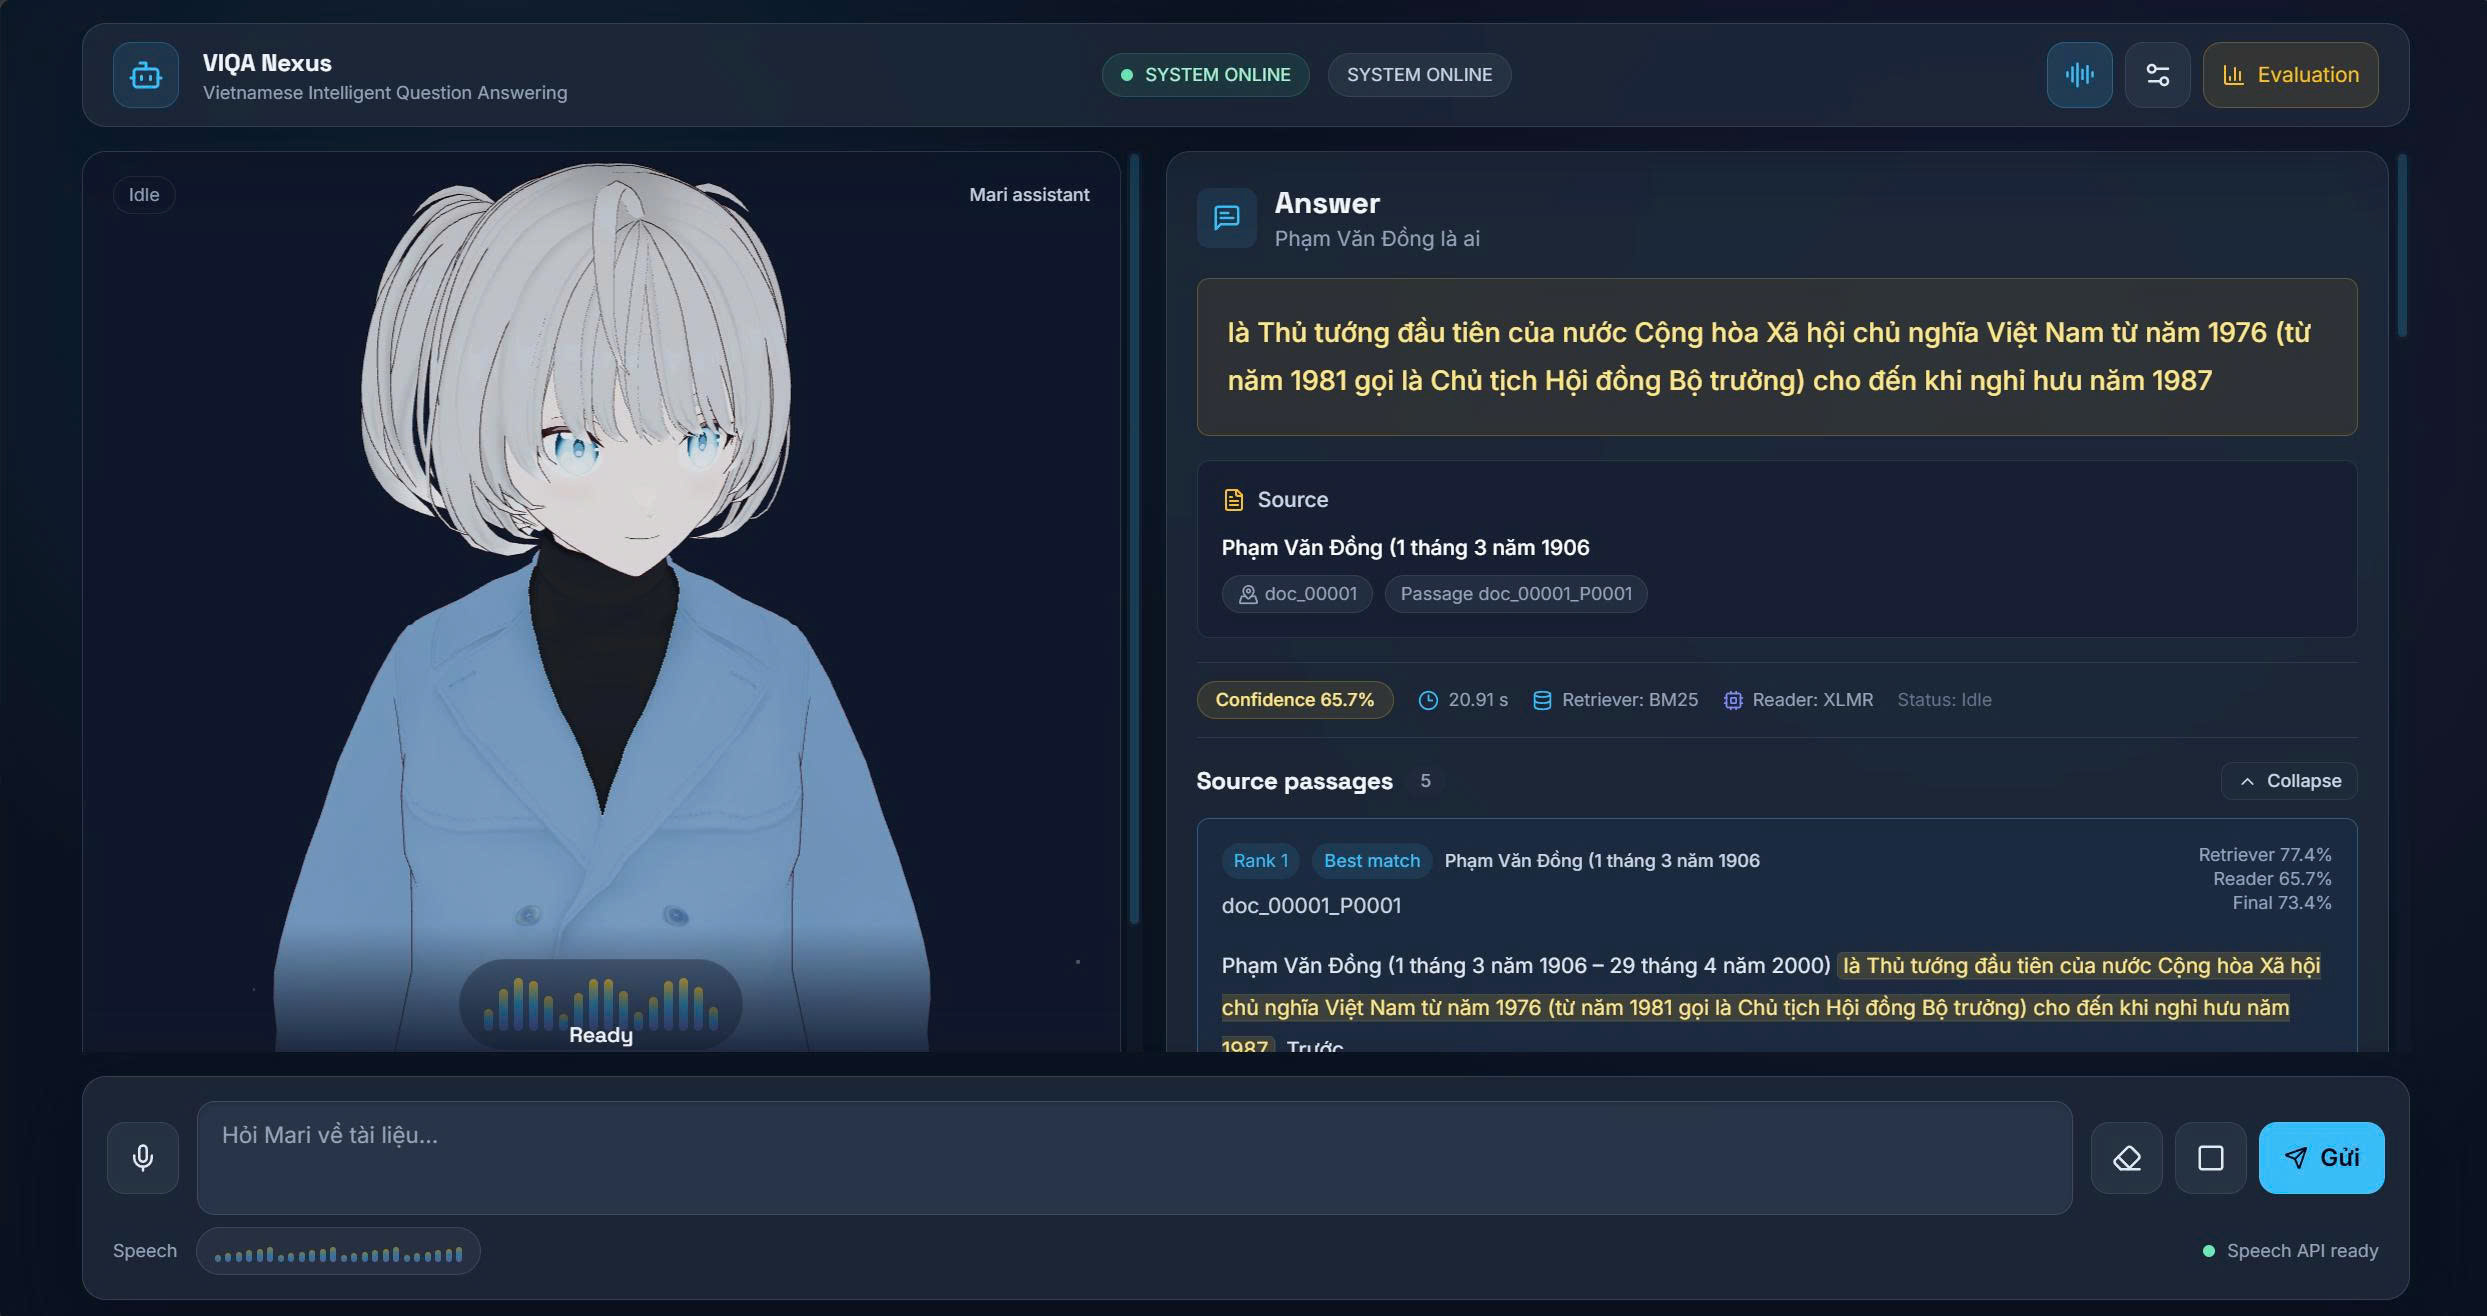
\includegraphics[width=0.95\textwidth]{UI_anw.jpg}
\caption{Answer Panel chi tiết kèm nguồn bằng chứng và chỉ số chẩn đoán}
\label{fig:answer-panel}
\end{figure}

\section{Avatar Mari và tương tác 3D}
Mari được tải từ tệp VRM bằng \texttt{@pixiv/three-vrm}. Scene hiện có blink, breathing,
expression, look-at theo chuột, spring-bone cho tóc và thinking pose đưa tay gần miệng. Pose
khởi tạo xoay model về camera và hạ tay khỏi T-pose. Avatar là lớp tương tác và trình bày;
nó không cải thiện Recall, EM hay F1 của pipeline NLP.

\begin{figure}[H]
\centering
\begin{tikzpicture}[node distance=1.2cm and 1.5cm]
\node[block, text width=2.8cm] (idle) {REST / IDLE\\(Blink, Breathing)};
\node[block, right=of idle, text width=2.8cm] (ret) {RETRIEVING\\(Head look-at)};
\node[block, below=of ret, text width=2.8cm] (think) {THINKING\\(Hand near mouth)};
\node[block, left=of think, text width=2.8cm] (speak) {SPEAKING\\(Lip-sync / Viseme)};

\draw[flowarrow] (idle) -- node[above, font=\tiny] {User Submit} (ret);
\draw[flowarrow] (ret) -- node[right, font=\tiny] {Top-$k$ Ready} (think);
\draw[flowarrow] (think) -- node[below, font=\tiny] {Span Extracted} (speak);
\draw[flowarrow] (speak) -- node[left, font=\tiny] {TTS Complete} (idle);
\end{tikzpicture}
\caption{Sơ đồ chuyển trạng thái tương tác của Avatar Mari 3D Humanoid}
\label{fig:mari-avatar}
\end{figure}

\section{Tương tác giọng nói}
Speech Recognition của trình duyệt nhận tiếng Việt với locale \texttt{vi-VN}; Speech
Synthesis đọc answer và ưu tiên giọng nữ nếu hệ điều hành/trình duyệt cung cấp. Việc lựa chọn
voice phụ thuộc danh sách voice của máy client, nên không thể bảo đảm cùng một giọng trên mọi
môi trường. Chuyển động miệng hiện dựa trên biên độ/timing cơ bản, chưa phải lip-sync theo
phoneme hoặc viseme. Đây là khác biệt quan trọng giữa hiệu ứng demo và đồng bộ khẩu hình thật.

\section{Hiển thị pipeline}
Pipeline panel ánh xạ trạng thái xử lý thành bốn bước Question, Retriever, Reader và Answer.
Kích thước từng bước được cố định để trạng thái và nhãn không làm layout dịch chuyển. Nội dung
UI dùng tiếng Anh thống nhất; thông báo chờ được chuẩn hóa thành ``Thinking about the
answer...'' và trạng thái chưa hỏi là ``Ask a question to begin.''.

\begin{figure}[H]
\centering
\begin{tikzpicture}[scale=0.95, transform shape]
\draw[fill=lightgray!20, draw=gray!30, rounded corners=6pt] (0,0) rectangle (13,2.2);

\node[draw=viqablue, fill=lightblue, rounded corners=4pt, text width=2.4cm, align=center, font=\sffamily\small] (step1) at (1.6,1.1) {\textbf{1. Question}\\\tiny Input Validation};
\node[draw=viqablue, fill=lightblue, rounded corners=4pt, text width=2.4cm, align=center, font=\sffamily\small] (step2) at (4.7,1.1) {\textbf{2. Retriever}\\\tiny BM25 Top-$k$};
\node[draw=viqablue, fill=lightblue, rounded corners=4pt, text width=2.4cm, align=center, font=\sffamily\small] (step3) at (7.8,1.1) {\textbf{3. Reader}\\\tiny PhoBERT Span};
\node[draw=viqablue, fill=lightblue, rounded corners=4pt, text width=2.4cm, align=center, font=\sffamily\small] (step4) at (10.9,1.1) {\textbf{4. Answer}\\\tiny Final Rerank};

\draw[flowarrow] (step1) -- (step2);
\draw[flowarrow] (step2) -- (step3);
\draw[flowarrow] (step3) -- (step4);
\end{tikzpicture}
\caption{Thanh hiển thị trạng thái xử lý 4 bước (Pipeline Visualization)}
\label{fig:pipeline-ui}
\end{figure}

\section{Compare Retriever}
Chế độ Compare Retriever gọi cùng câu hỏi với TF--IDF và BM25 rồi đặt kết quả cạnh nhau để
so sánh passage, score và thời gian. Dense/Pyserini không được trình bày như lựa chọn chạy thật
trong màn hình này cho đến khi API hỗ trợ. So sánh một truy vấn giúp phân tích định tính nhưng
không thay thế benchmark nhiều câu hỏi.

\begin{figure}[H]
\centering
\begin{subfigure}[t]{0.49\textwidth}
\centering
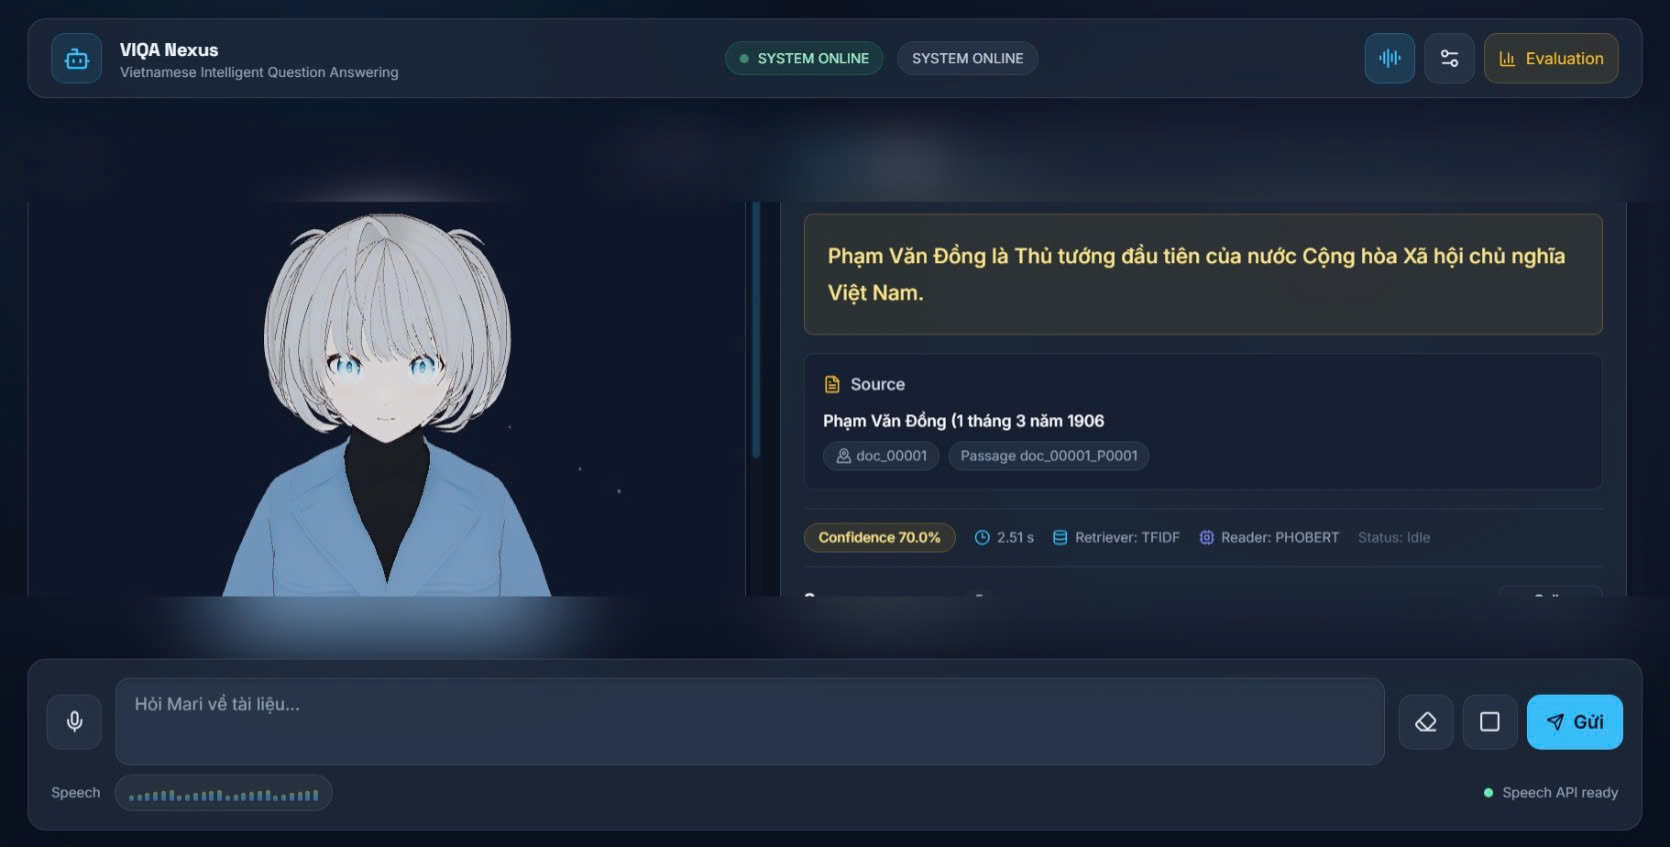
\includegraphics[width=\textwidth]{TFIDF.jpg}
\caption{TF--IDF}
\end{subfigure}
\hfill
\begin{subfigure}[t]{0.49\textwidth}
\centering
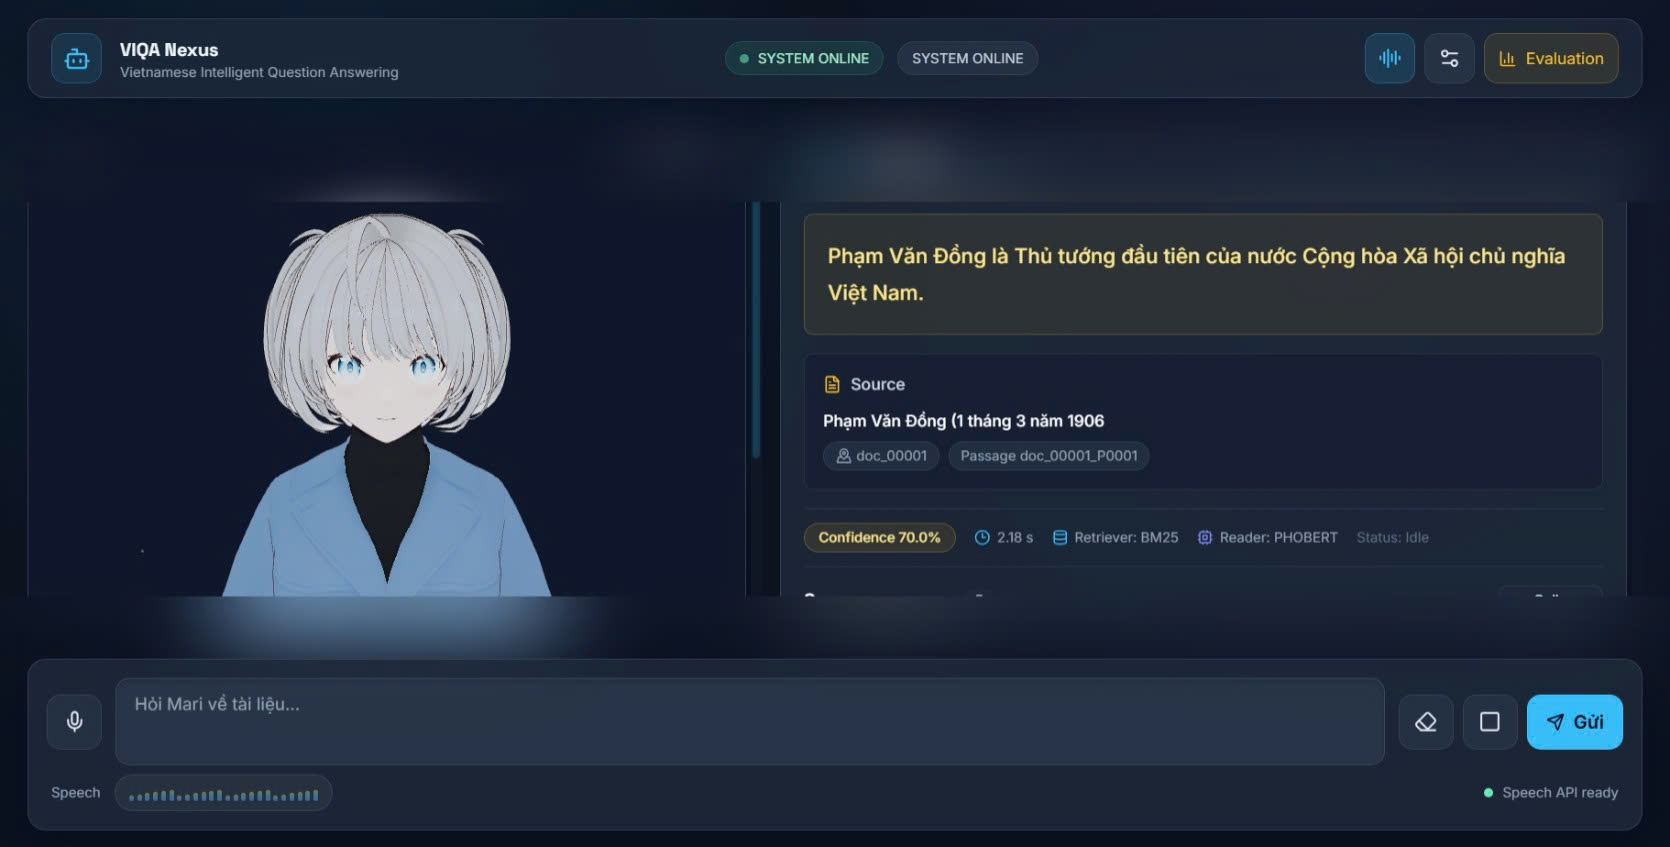
\includegraphics[width=\textwidth]{BM25.jpg}
\caption{BM25}
\end{subfigure}
\caption{Giao diện so sánh song song kết quả truy hồi giữa TF-IDF và BM25}
\label{fig:compare-ui}
\end{figure}

\section{Evaluation page}
Trang Evaluation hiện là giao diện mock nhằm minh họa bảng và biểu đồ dự kiến; nó chưa đọc
trực tiếp các artifact benchmark trong \texttt{results/}. Vì vậy số liệu học thuật trong báo
cáo lấy từ file kết quả thật, không lấy từ UI mock. Hướng hoàn thiện là thêm endpoint đọc JSON
benchmark, hiển thị provenance, timestamp và cấu hình chạy.

\begin{figure}[H]
\centering
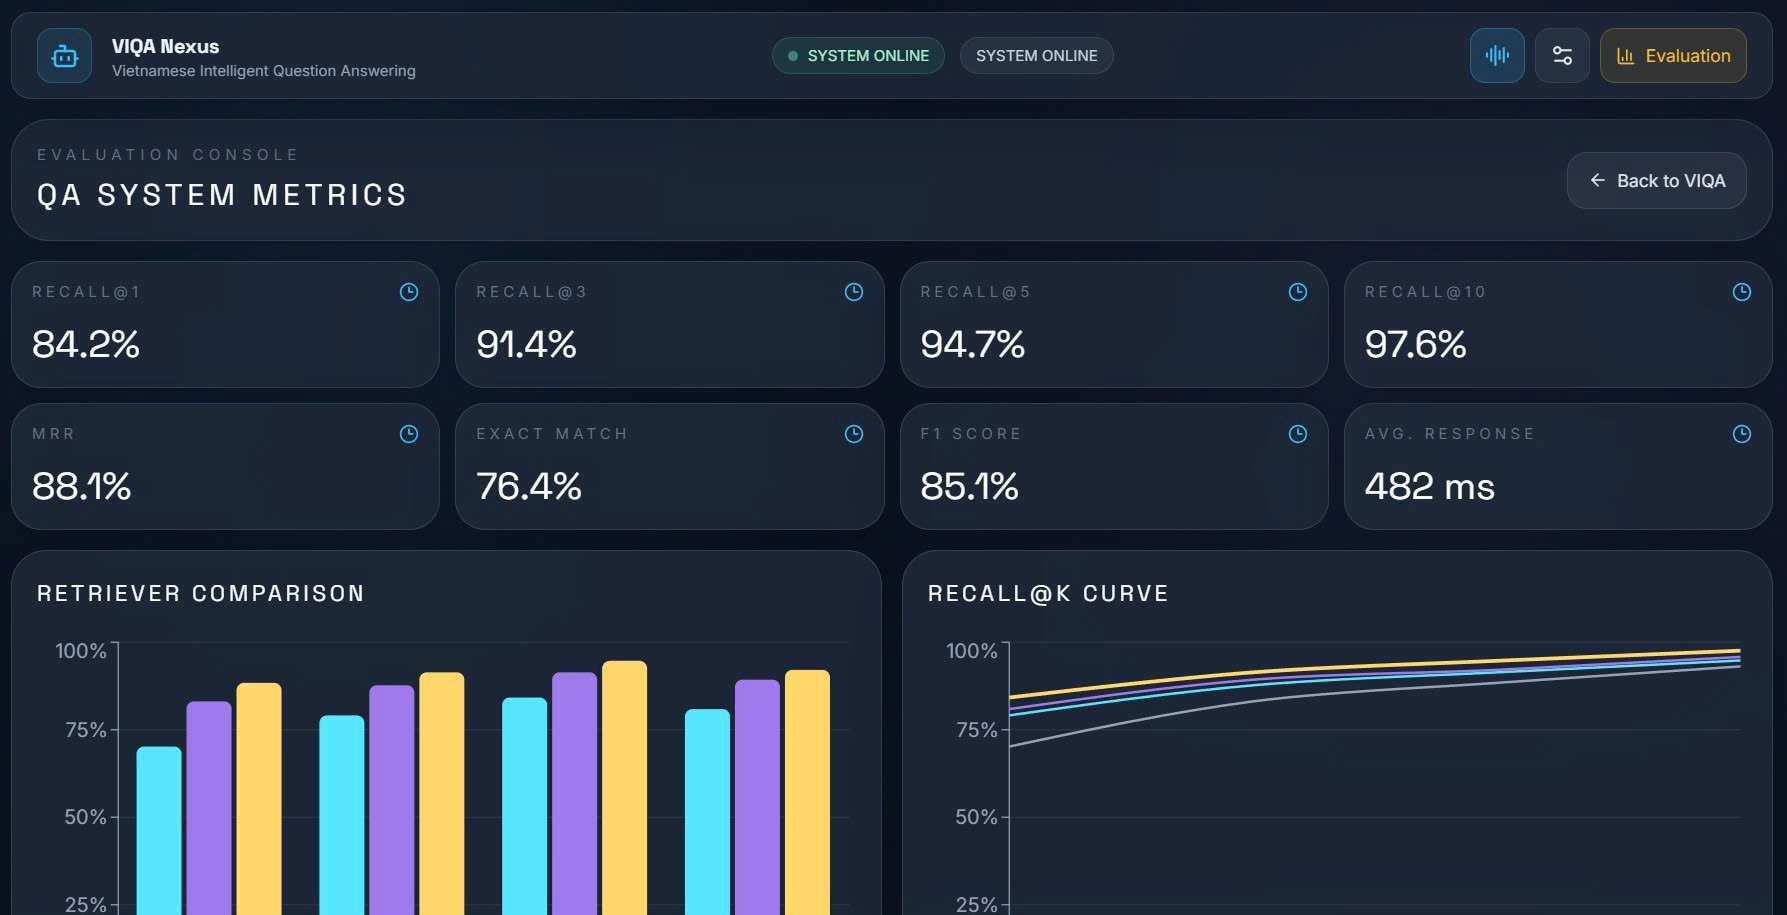
\includegraphics[width=0.95\textwidth]{dashboard.jpg}
\caption{Màn hình Evaluation Dashboard hiển thị provenance kết quả thực nghiệm}
\label{fig:evaluation-ui}
\end{figure}

\chapter{Thực nghiệm và đánh giá}
\label{chap:experiments}

\section{Mục tiêu và câu hỏi thực nghiệm}
Thực nghiệm được tổ chức để trả lời bốn câu hỏi. Thứ nhất, Retriever nào tìm được passage
đúng tốt nhất trên corpus hiện tại? Thứ hai, chi phí truy vấn của từng phương pháp khác nhau
ra sao? Thứ ba, PhoBERT Reader có trích xuất được answer span khi được cung cấp oracle
context hay không? Thứ tư, pipeline hoàn chỉnh đạt EM, F1 và latency nào khi context đến từ
Retriever? Các kết quả được báo cáo theo từng tầng để phân biệt chất lượng retrieval, Reader
oracle và end-to-end.

\section{Môi trường thực nghiệm}
\begin{table}[H]
\centering
\caption{Môi trường phần cứng và phần mềm đã ghi nhận}
\label{tab:environment}
\begin{tabularx}{\textwidth}{|L{0.31\textwidth}|Y|}
\hline
Thành phần & Cấu hình \\
\hline
Hệ điều hành & Windows 11 x64, build 22621 \\
\hline
CPU & Intel Core i5-13420H \\
\hline
RAM & 15,73 GB \\
\hline
GPU vật lý & NVIDIA GeForce RTX 3050 Laptop, 6 GB \\
\hline
Python & 3.12.0 \\
\hline
Node.js / npm & 22.16.0 / 10.9.2 \\
\hline
PyTorch & 2.11.0+cpu \\
\hline
Transformers & 4.57.6 \\
\hline
CUDA khi chạy benchmark & Không; PyTorch build CPU \\
\hline
\end{tabularx}
\end{table}

Mặc dù máy có GPU rời, bản PyTorch đang dùng là CPU-only. Do đó latency Reader trong môi
trường này không phản ánh khả năng tăng tốc CUDA. Khi so sánh lại sau này phải ghi rõ device,
batch size, sequence length, warm-up và số lần lặp; nếu thiếu các điều kiện này, so sánh thời
gian giữa hai máy không có ý nghĩa.

\section{Thiết lập đánh giá Retriever}
Mỗi câu hỏi test được gắn với document/context chứa đáp án. Retriever trả danh sách passage
đã sắp hạng; một hit xảy ra khi passage đúng xuất hiện trong top-$k$. Các metric Recall@1,
Recall@3, Recall@5, Recall@10 và MRR được tính theo \cref{eq:recall-k,eq:mrr}. QPS đo số truy
vấn xử lý trong một giây ở benchmark retrieval, không gồm thời gian neural Reader, HTTP hay
render frontend.

Do passage runtime được tạo từ document context, script đánh giá phải dùng cùng quy tắc ánh
xạ positive passage cho cả ba phương pháp. Nếu một phương pháp dùng corpus/index khác, số liệu
không còn so sánh trực tiếp. Các kết quả dưới đây được lấy từ artifact đã lưu trong
\texttt{results/}; báo cáo không suy diễn độ lệch chuẩn vì chưa có nhiều lần chạy độc lập.

\section{Kết quả Retriever}
\begin{table}[H]
\centering
\caption{Kết quả Retriever trên tập test UIT-ViQuAD2.0}
\label{tab:retriever-results}
\begin{tabular}{|l|r|r|r|r|r|r|}
\hline
Phương pháp & R@1 (\%) & R@3 (\%) & R@5 (\%) & R@10 (\%) & MRR (\%) & QPS \\
\hline
TF--IDF & 55,47 & 71,20 & 76,55 & 83,21 & 65,17 & \textbf{657,8} \\
\hline
BM25 & \textbf{59,39} & \textbf{74,33} & \textbf{79,50} & \textbf{85,15} & \textbf{68,50} & 33,7 \\
\hline
Dense & 31,79 & 47,03 & 53,99 & 63,66 & 42,25 & 166,6 \\
\hline
\end{tabular}
\end{table}

BM25 đạt kết quả cao nhất ở mọi mức Recall và MRR. So với TF--IDF, BM25 tăng 3,92 điểm phần
trăm ở R@1, 2,95 ở R@5 và 3,33 ở MRR. Điều này phù hợp với lợi ích của saturation và length
normalization trên các passage có độ dài không hoàn toàn đồng nhất. Tuy vậy, TF--IDF nhanh
hơn khoảng 19,5 lần theo QPS đã ghi nhận. Vì Reader thường là nút thắt thời gian lớn hơn, lựa
chọn cuối không thể chỉ dựa trên QPS retrieval; cần đo latency end-to-end.

Dense thấp hơn BM25 27,60 điểm phần trăm ở R@1 và 25,25 ở MRR. Kết quả này không chứng minh
dense retrieval nói chung kém sparse retrieval. Nó chỉ cho thấy cấu hình Dense hiện tại,
chưa fine-tune theo miền và dữ liệu câu hỏi--passage tiếng Việt của project, chưa cạnh tranh
được. Sentence embedding tổng quát có thể gom gần nội dung cùng chủ đề nhưng chưa tối ưu để
đưa đúng passage chứa answer span lên đầu.

\begin{figure}[H]
\centering
\begin{tikzpicture}
\begin{axis}[
  ybar,
  width=0.88\textwidth,
  height=7.0cm,
  ymin=0,ymax=100,
  ylabel={Tỷ lệ (\%)},
  symbolic x coords={TF--IDF,BM25,Dense},
  xtick=data,
  bar width=8pt,
  legend style={at={(0.5,-0.18)},anchor=north,legend columns=5},
  nodes near coords,
  every node near coord/.append style={font=\scriptsize,rotate=90,anchor=west},
  enlarge x limits=0.22
]
\addplot coordinates {(TF--IDF,55.47) (BM25,59.39) (Dense,31.79)};
\addplot coordinates {(TF--IDF,71.20) (BM25,74.33) (Dense,47.03)};
\addplot coordinates {(TF--IDF,76.55) (BM25,79.50) (Dense,53.99)};
\addplot coordinates {(TF--IDF,83.21) (BM25,85.15) (Dense,63.66)};
\addplot coordinates {(TF--IDF,65.17) (BM25,68.50) (Dense,42.25)};
\legend{R@1,R@3,R@5,R@10,MRR}
\end{axis}
\end{tikzpicture}
\caption{So sánh Recall@k và MRR của ba Retriever}
\label{fig:retriever-chart}
\end{figure}

Khoảng cách R@1 đến R@10 cho thấy tăng $k$ vẫn cứu được nhiều truy vấn. Với BM25, Recall
tăng từ 59,39\% lên 85,15\%, nghĩa là có khoảng 25,76 điểm phần trăm trường hợp positive nằm
ở hạng 2--10. Reader và reranker có cơ hội tận dụng phần này, nhưng cũng phải xử lý nhiều
distractor. Khoảng 14,85\% còn lại không có positive trong top 10 theo tiêu chí benchmark;
Reader không thể trích đúng answer từ một context không được truy hồi.

\begin{figure}[H]
\centering
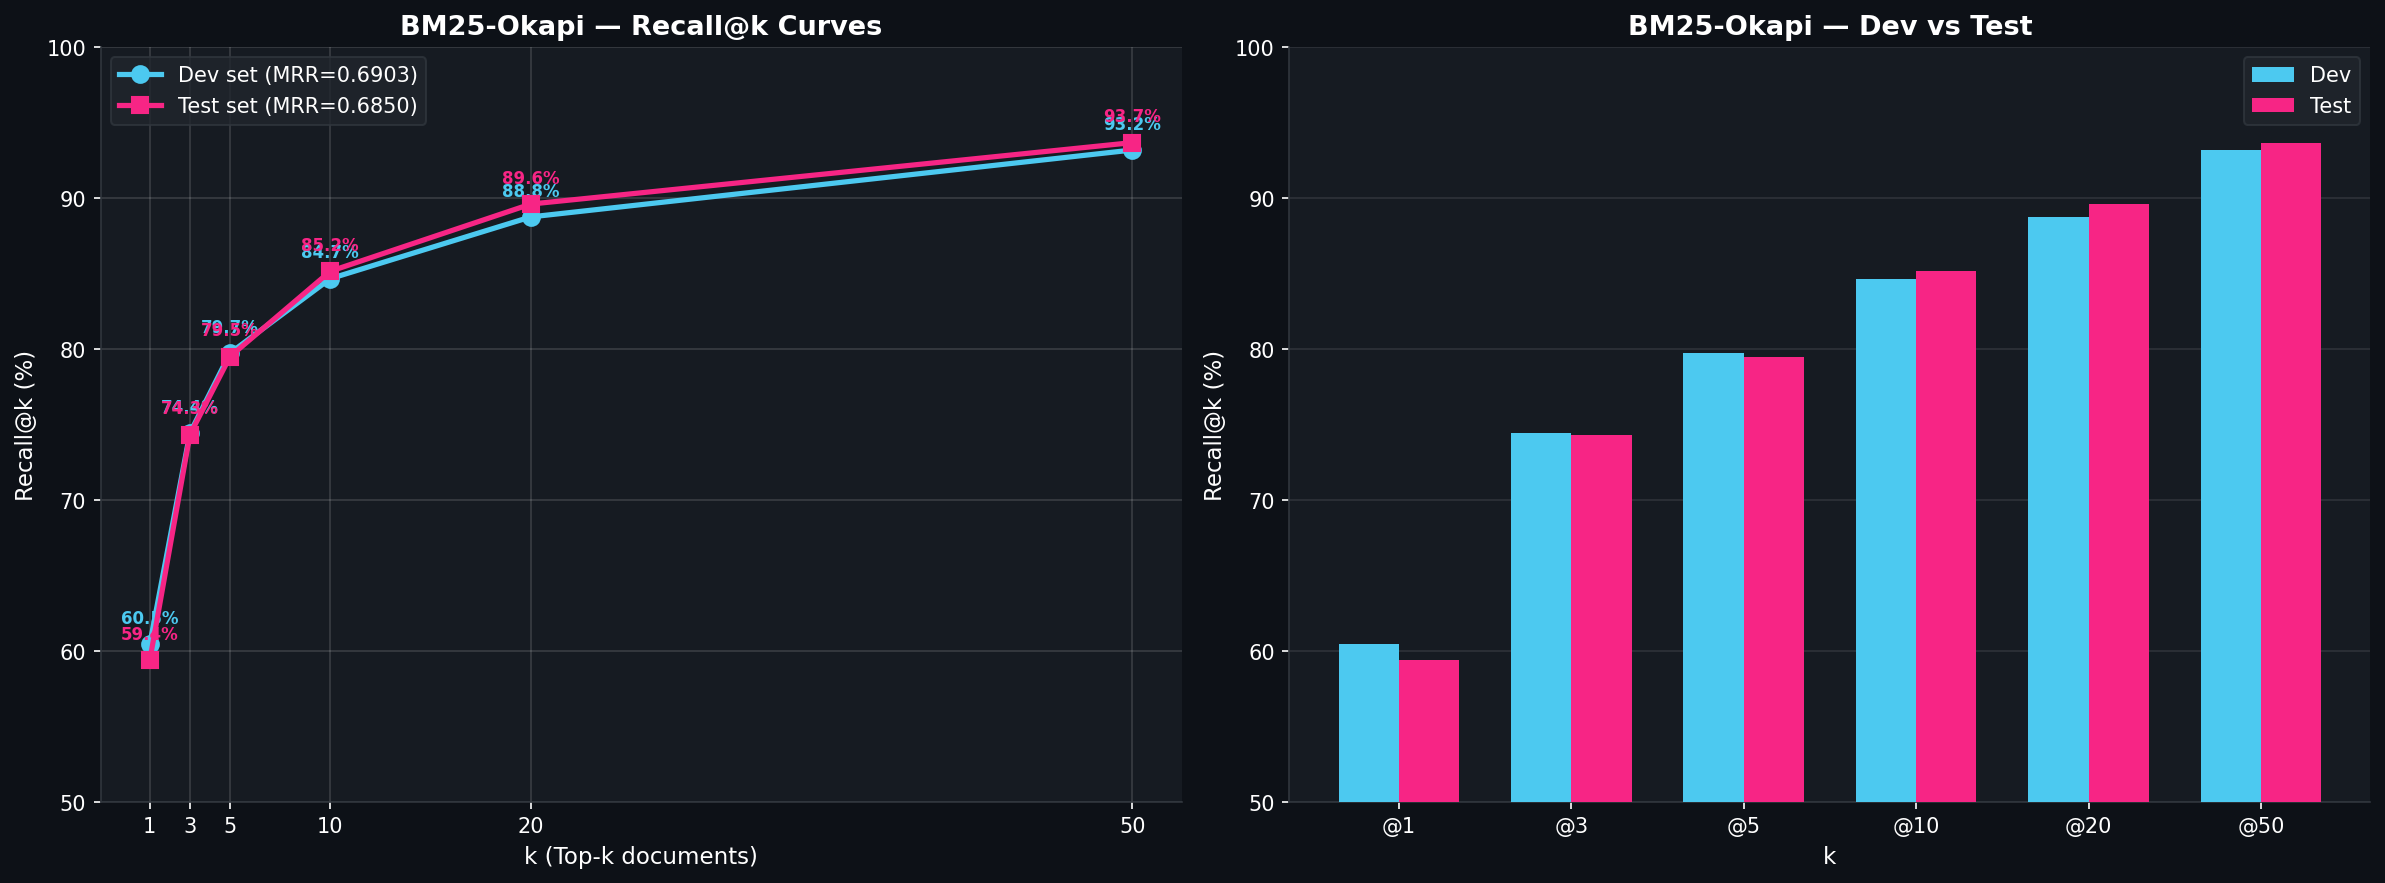
\includegraphics[width=0.85\textwidth]{bm25_retrieval_results.png}
\caption{Kết quả benchmark chi tiết của bộ truy hồi BM25 trên các tập dữ liệu}
\label{fig:retrieval-benchmark}
\end{figure}

\section{Thiết lập đánh giá Reader}
Reader được đánh giá ở chế độ oracle context trên 3.814 mẫu dev. Trong chế độ này, context
gốc có nhãn được đưa trực tiếp cho model, loại bỏ lỗi Retriever. EM và token-level F1 được
tính trên answer text sau chuẩn hóa. Kết quả tách answerable và unanswerable là bắt buộc vì một
mô hình luôn dự đoán no-answer có thể đạt điểm tổng thể gây hiểu nhầm khi tập dev có nhiều câu
không trả lời được.

\begin{figure}[H]
\centering
\begin{tikzpicture}[scale=0.9, transform shape]
\begin{axis}[
    title={Quá trình huấn luyện PhoBERT Reader (5 Epochs)},
    xlabel={Training Step},
    ylabel={Loss},
    xmin=0, xmax=4500,
    ymin=0, ymax=4.0,
    grid=major,
    legend pos=north east,
    width=12cm, height=6.5cm
]
\addplot[color=viqablue, mark=none, thick] coordinates {
    (0, 3.8) (500, 2.4) (1000, 1.8) (1500, 1.3) (2000, 0.95) (2500, 0.72) (3000, 0.54) (3500, 0.41) (4000, 0.33) (4500, 0.28)
};
\addplot[color=E76F51, mark=square*, thick] coordinates {
    (500, 2.9) (1500, 2.1) (2500, 1.85) (3500, 1.78) (4500, 1.76)
};
\legend{Training Loss, Validation Loss}
\end{axis}
\end{tikzpicture}
\caption{Biểu đồ theo dõi Loss trong quá trình fine-tune PhoBERT Reader trên UIT-ViQuAD2.0}
\label{fig:reader-training}
\end{figure}

\section{Kết quả Reader}
\begin{table}[H]
\centering
\caption{Kết quả PhoBERT Reader trên oracle context, dev 3.814 mẫu}
\label{tab:reader-results}
\begin{tabularx}{\textwidth}{|L{0.28\textwidth}|C{0.17\textwidth}|C{0.17\textwidth}|Y|}
\hline
Nhóm & EM (\%) & F1 (\%) & Diễn giải \\
\hline
Toàn bộ dev & 28,68 & 29,46 & Bị chi phối bởi khả năng nhận no-answer \\
\hline
Answerable & 0,30 & 1,42 & Trích span có đáp án rất yếu \\
\hline
Unanswerable & 93,54 & -- & Mô hình thường nhận đúng no-answer \\
\hline
\end{tabularx}
\end{table}

Kết quả này chưa đạt yêu cầu cho một Reader sản phẩm. Khi đã có oracle context mà F1 trên
answerable chỉ 1,42\%, nguồn lỗi chính không thể quy hoàn toàn cho Retriever. EM tổng thể
28,68\% không nên được gọi là ``khá'' hay ``ổn định'', bởi nó che giấu sự mất cân bằng giữa
hai nhóm. EM unanswerable 93,54\% cho thấy mô hình học hoặc được hiệu chỉnh theo hướng từ chối
rất mạnh; chính hành vi đó có thể làm câu hỏi phổ biến như ``Phạm Văn Đồng là ai?'' nhận thông
báo không tìm thấy dù passage phù hợp đã xuất hiện.

Các giả thuyết cần kiểm chứng gồm: tỷ lệ answerable/unanswerable trong batch; cách ánh xạ
answer start sau word segmentation; nhãn CLS/no-answer; truncation làm mất span; learning
rate và số epoch; checkpoint 4.500 chưa phải checkpoint tốt nhất; hoặc lỗi chuẩn hóa khi tính
metric. Không giả thuyết nào được kết luận là nguyên nhân nếu chưa có thống kê alignment và
ablation. Bước kiểm tra đầu tiên nên là cho model overfit một tập rất nhỏ 32--100 mẫu
answerable. Nếu không overfit được, lỗi nằm ở data/label/loss hoặc code training; nếu overfit
được, mới mở rộng sang sampling, hyperparameter và calibration.

\section{Đánh giá end-to-end}
Đánh giá end-to-end phải dùng retrieved context thay vì oracle context. Một prediction chỉ
đúng khi Retriever đưa bằng chứng phù hợp và Reader/fallback chọn đúng answer. Cần chạy riêng
TF--IDF+PhoBERT và BM25+PhoBERT, đồng thời tách method neural/fallback và thống kê no-answer.
Kết quả hiện có được tổng hợp trong \cref{tab:end-to-end-results}.

\begin{table}[H]
\centering
\scriptsize
\caption{Kết quả end-to-end}
\label{tab:end-to-end-results}
\begin{tabularx}{\textwidth}{|L{0.29\textwidth}|C{0.16\textwidth}|C{0.16\textwidth}|C{0.18\textwidth}|Y|}
\hline
Cấu hình & EM (\%) & F1 (\%) & Latency & Ghi chú \\
\hline
TF--IDF + PhoBERT & 1,00 & 2,96 & 2204,89 ms & Retrieved context \\
\hline
BM25 + PhoBERT & 0,00 & 1,00 & 2027,50 ms & Retrieved context \\
\hline
BM25 + PhoBERT + fallback & 0,00 & 4,50 & 2377,73 ms & Tách tỷ lệ fallback (PhoBERT: 0,0\%, Fallback: 100,0\%) \\
\hline
\end{tabularx}
\end{table}

Các giá trị latency trong bảng là thời gian xử lý ghi nhận theo cấu hình đánh giá tương ứng.
Nếu mở rộng benchmark, script nên khóa tập test, seed, index version, checkpoint hash và cấu
hình threshold; warm-up trước khi đo latency; báo cáo thêm median, mean và p95 thay vì chỉ một
giá trị tổng hợp.

\section{Phân tích lỗi}
Do chưa có file prediction end-to-end được gắn nhãn lỗi, bảng dưới đây trình bày taxonomy và
quy trình xác minh, không bịa số ca. Mỗi prediction cần lưu question ID, gold answers,
retrieved IDs/scores, predicted span, null score, final score và method.

\begin{table}[H]
\centering
\caption{Khung phân tích lỗi end-to-end}
\label{tab:error-analysis}
\begin{tabularx}{\textwidth}{|L{0.20\textwidth}|Y|L{0.22\textwidth}|L{0.20\textwidth}|}
\hline
Nhóm lỗi & Dấu hiệu phân loại & Số trường hợp & Hướng kiểm tra \\
\hline
Retriever miss & Gold passage không có trong top 10 & -- & Query terms, chunk/index \\
\hline
Reader no-answer sai & Gold passage có, model chọn null & -- & Null margin, threshold, labels \\
\hline
Span boundary sai & Có overlap với gold nhưng EM sai & -- & Offset/alignment, punctuation \\
\hline
Distractor thắng & Passage sai có final score cao hơn & -- & Reranking và calibration \\
\hline
Fallback dư ý & Câu có answer nhưng chứa mệnh đề thừa & -- & Sentence selection/postprocess \\
\hline
Fallback sai nghĩa & Có entity nhưng không trả lời quan hệ hỏi & -- & Question type/semantic filter \\
\hline
Gold ambiguity & Nhiều cách trả lời hợp lệ & -- & Review thủ công và aliases \\
\hline
Latency outlier & Thời gian vượt p95 mục tiêu & -- & Windows, batch, cold start \\
\hline
\end{tabularx}
\end{table}

Ví dụ câu hỏi ``Phạm Văn Đồng là ai?'' nên được phân tích theo trình tự: kiểm tra BM25 có đưa
passage tiểu sử vào top-$k$; kiểm tra neural Reader chọn null hay span; nếu fallback chạy, xác
nhận câu được chọn có mô tả vai trò của nhân vật thay vì quan hệ gia đình; cuối cùng kiểm tra
reranker có đặt passage định nghĩa lên trên passage chỉ nhắc tên. Cách phân tầng này tránh sửa
post-processing khi lỗi thực tế nằm ở corpus hoặc Reader.

\section{Thảo luận kết quả}
Kết quả retrieval đủ để kết luận BM25 là baseline phù hợp nhất trong ba cấu hình đã benchmark
cho corpus hiện tại. TF--IDF vẫn có giá trị khi cần tốc độ và làm đối chứng đơn giản. Dense
cần fine-tune và đánh giá lại trước khi tích hợp, thay vì được chọn chỉ vì là phương pháp mới
hơn. Pyserini cần index tái tạo được và benchmark cùng protocol.

Đối với Reader, dữ liệu hiện tại chỉ hỗ trợ kết luận rằng checkpoint có thiên lệch no-answer
nghiêm trọng. Fallback cải thiện trải nghiệm ở một số truy vấn nhưng không thay thế việc sửa
Reader. Kết quả end-to-end hiện tại còn thấp, đặc biệt EM chỉ đạt 0--1\% và F1 cao nhất đạt
4,50\% ở cấu hình có fallback, nên chưa thể xem hệ thống là một sản phẩm QA chính xác.

Các metric cũng phản ánh các tầng khác nhau. Recall/MRR đo khả năng mang bằng chứng đến
Reader; oracle EM/F1 đo Reader trong điều kiện lý tưởng; end-to-end EM/F1 đo sản phẩm kết hợp;
latency đo khả năng sử dụng. Chỉ báo cáo một tầng sẽ dẫn đến kết luận thiếu: Recall tốt không
bảo đảm answer tốt, còn oracle Reader tốt cũng vô dụng nếu Retriever bỏ lỡ passage.

\chapter{Kết luận và hướng phát triển}
\label{chap:conclusion}

\section{Kết quả đạt được}
Đề tài đã xây dựng được một prototype hỏi đáp trích xuất tiếng Việt theo kiến trúc
Retriever--Reader. Corpus và ba split QA được chuẩn hóa từ UIT-ViQuAD2.0; tài liệu được chia
thành passage có overlap và lưu bằng định danh truy vết được. Hai sparse Retriever TF--IDF,
BM25 hoạt động trong API; Dense Retrieval và Pyserini có implementation ở mức offline/thử
nghiệm. PhoBERT QA checkpoint được tích hợp với start/end logits, offset mapping, sliding
window, batch inference, no-answer và fallback.

Về thực nghiệm, project đã có benchmark retrieval trên test cho ba phương pháp và đánh giá
Reader oracle trên dev. BM25 dẫn đầu retrieval với R@5 79,50\% và MRR 68,50\%; TF--IDF có
QPS cao nhất. Reader hiện chưa đạt yêu cầu trên câu answerable, một phát hiện quan trọng để
định hướng công việc tiếp theo. Báo cáo không che khuất vấn đề này bằng điểm unanswerable cao
và ghi nhận kết quả end-to-end còn thấp để định hướng cải tiến.

Prototype giao diện React tích hợp avatar Mari 3D, nhập giọng nói, đọc câu trả lời, hiển thị
pipeline, nguồn và so sánh Retriever. Các thành phần này làm hệ thống dễ trình diễn và dễ quan
sát, nhưng đóng góp NLP cốt lõi vẫn là dữ liệu, retrieval, reading và quy trình đánh giá.

\section{Hạn chế}
\begin{table}[H]
\centering
\footnotesize
\caption{Các hạn chế hiện tại của VIQA Nexus}
\label{tab:limitations}
\begin{tabularx}{\textwidth}{|L{0.21\textwidth}|Y|L{0.27\textwidth}|}
\hline
Thành phần & Hạn chế & Ảnh hưởng \\
\hline
Dữ liệu & Corpus chỉ phản ánh context của UIT-ViQuAD2.0, chưa phải toàn bộ Wikipedia & Miền tri thức và độ bao phủ bị giới hạn \\
\hline
Chunking & Kích thước 220 token, overlap 2 chưa có ablation & Có thể bỏ mất quan hệ hoặc tăng distractor \\
\hline
TF--IDF/BM25 & Dựa mạnh vào lexical overlap & Yếu với paraphrase và đồng nghĩa \\
\hline
Dense & Chưa fine-tune theo miền; chưa nối API & Chất lượng thấp và chưa dùng trong sản phẩm \\
\hline
Pyserini & Thiếu index/benchmark chính thức/API & Chưa tái lập đầy đủ end-to-end \\
\hline
Reader & Answerable EM/F1 rất thấp, lệch no-answer & Bỏ từ chối hoặc trích sai dù context đúng \\
\hline
Reranking & Trọng số cấu hình chưa tuning/calibration & Final score chưa có ý nghĩa xác suất \\
\hline
Fallback & Có thể trả câu dư ý hoặc không đúng quan hệ & Answer dễ đọc nhưng chưa chắc chính xác \\
\hline
Đánh giá & Chưa có prediction log gắn nhãn lỗi đầy đủ & Chưa phân tích được nguyên nhân lỗi end-to-end theo taxonomy \\
\hline
Runtime & PyTorch CPU; server demo đơn giản & Latency cao và khả năng phục vụ hạn chế \\
\hline
UI & Evaluation còn mock; lip-sync mức biên độ & Một số hiển thị chưa phản ánh backend thật \\
\hline
\end{tabularx}
\end{table}

Ngoài ra, dataset có cả câu không trả lời được nên metric tổng thể nhạy với phân bố lớp. Một
model có thể tăng EM bằng cách từ chối nhiều hơn mà giảm mạnh ích lợi thực tế. Mọi lần đánh
giá tiếp theo cần công bố kết quả answerable, unanswerable và overall riêng, kèm confusion
matrix của quyết định no-answer.

\section{Hướng phát triển}
\begin{table}[H]
\centering
\footnotesize
\caption{Lộ trình cải tiến đề xuất}
\label{tab:future-work}
\begin{tabularx}{\textwidth}{|C{0.08\textwidth}|L{0.22\textwidth}|Y|L{0.22\textwidth}|}
\hline
Ưu tiên & Hạng mục & Công việc cụ thể & Tiêu chí hoàn thành \\
\hline
P0 & Sửa Reader & Audit alignment; overfit tập nhỏ; cân bằng answerable; kiểm tra loss/CLS; chọn checkpoint & Answerable EM/F1 tăng trên dev cố định \\
\hline
P0 & End-to-end eval & Lưu predictions; tách neural/fallback; đo mean/median/p95 & Điền Bảng~\ref{tab:end-to-end-results} tái lập được \\
\hline
P1 & Threshold/calibration & Tune no-answer và final score trên dev; reliability curve & Giảm false no-answer, không dùng test để tune \\
\hline
P1 & Retrieval hybrid & Kết hợp BM25 và Dense bằng RRF hoặc score fusion & R@k/MRR cao hơn BM25 có ý nghĩa \\
\hline
P1 & Dense fine-tuning & Huấn luyện multilingual-E5/Sentence Transformer với hard negatives & Dense vượt baseline hiện tại \\
\hline
P1 & Reranker & Cross-encoder xếp lại top candidates & Tăng end-to-end F1 trong ngân sách latency \\
\hline
P2 & Pyserini & Script build Lucene index, pin version, benchmark và API adapter & Tái tạo index bằng một lệnh \\
\hline
P2 & Tăng tốc & CUDA build, batch, cache index/model, profiling & Giảm p50/p95 trên cùng phần cứng \\
\hline
P2 & API & Cân nhắc FastAPI, schema validation, async job cho benchmark & API có contract và health/readiness rõ \\
\hline
P3 & UI Evaluation & Đọc artifact thật và provenance từ backend & Không còn metric mock \\
\hline
P3 & Voice/avatar & Phoneme/viseme lip-sync, fallback voice rõ ràng & Khẩu hình ổn định, không ảnh hưởng QA \\
\hline
\end{tabularx}
\end{table}

Thứ tự P0 ưu tiên độ đúng trước tốc độ và hiệu ứng giao diện. Reader cần được kiểm tra bằng
unit test dữ liệu: answer substring phải khớp offset trước và sau segmentation; feature chứa
answer phải có start/end label hợp lệ; feature không chứa answer phải gán null đúng. Sau đó
chạy overfit nhỏ, huấn luyện lại với logging đầy đủ và chọn threshold trên dev. Đây là đường
ngắn nhất để phân biệt lỗi code với giới hạn mô hình.

Với retrieval, một hướng ít rủi ro là Reciprocal Rank Fusion giữa BM25 và Dense đã fine-tune:
\begin{equation}
\operatorname{RRF}(d)=\sum_{r\in\mathcal{R}}\frac{1}{K+\operatorname{rank}_r(d)},
\end{equation}
trong đó $\mathcal{R}$ là tập Retriever và $K$ là hằng số làm trơn được chọn trên dev. Sau
fusion, cross-encoder có thể xếp lại top 20--50 passage trước khi gửi 5 passage tốt nhất cho
Reader. Mỗi tầng chỉ nên được giữ nếu ablation cho thấy tăng end-to-end F1 đủ bù latency.

Việc dùng LLM có thể là pha sau: tạo câu trả lời diễn đạt từ bằng chứng đã truy hồi hoặc kiểm
tra tính đầy đủ. Tuy nhiên LLM không thay thế corpus, retrieval và benchmark; nếu đưa vào,
prompt phải buộc trích dẫn passage, có chế độ từ chối và đánh giá hallucination. Với mục tiêu
môn học NLP hiện tại, sửa Reader và hoàn thiện end-to-end evaluation mang giá trị khoa học rõ
hơn việc thêm một API sinh văn bản ngay lập tức.

\section{Kết luận}
VIQA Nexus cho thấy một hệ thống QA có thể được xây dựng theo module, quan sát được và mở rộng
được từ baseline DrQA sang tiếng Việt. Giá trị của prototype không chỉ nằm ở giao diện 3D mà
ở khả năng đối chiếu Retriever, Reader và nguồn passage. Benchmark cho thấy BM25 là lựa chọn
retrieval tốt nhất hiện tại, đồng thời phơi bày Reader là nút thắt chất lượng cần xử lý.

Kết luận trung thực của đề tài là hệ thống đã chạy được end-to-end ở mức prototype nhưng độ
chính xác hiện còn thấp. Các số liệu chưa có artifact được đánh dấu ``--'' để phân biệt rõ
phần đã đo được với phần chưa đủ dữ liệu. Khi Reader answerable được sửa, score được
calibration và prediction log end-to-end được phân tích theo taxonomy lỗi, project sẽ có nền
tảng vững hơn để mở rộng sang hybrid retrieval, reranking và trả lời sinh có căn cứ.

\clearpage
\addcontentsline{toc}{chapter}{Tài liệu tham khảo}
\begin{thebibliography}{99}

\bibitem{drqa}
Danqi Chen, Adam Fisch, Jason Weston, and Antoine Bordes.
\newblock Reading Wikipedia to Answer Open-Domain Questions.
\newblock In \emph{Proceedings of the 55th Annual Meeting of the Association for
Computational Linguistics}, pages 1870--1879, 2017.
\newblock DOI: \url{https://doi.org/10.18653/v1/P17-1171}.

\bibitem{transformer}
Ashish Vaswani, Noam Shazeer, Niki Parmar, Jakob Uszkoreit, Llion Jones,
Aidan N. Gomez, Lukasz Kaiser, and Illia Polosukhin.
\newblock Attention Is All You Need.
\newblock In \emph{Advances in Neural Information Processing Systems 30}, 2017.

\bibitem{bert}
Jacob Devlin, Ming-Wei Chang, Kenton Lee, and Kristina Toutanova.
\newblock BERT: Pre-training of Deep Bidirectional Transformers for Language Understanding.
\newblock In \emph{Proceedings of NAACL-HLT}, pages 4171--4186, 2019.
\newblock DOI: \url{https://doi.org/10.18653/v1/N19-1423}.

\bibitem{roberta}
Yinhan Liu, Myle Ott, Naman Goyal, Jingfei Du, Mandar Joshi, Danqi Chen,
Omer Levy, Mike Lewis, Luke Zettlemoyer, and Veselin Stoyanov.
\newblock RoBERTa: A Robustly Optimized BERT Pretraining Approach.
\newblock arXiv preprint arXiv:1907.11692, 2019.

\bibitem{phobert}
Dat Quoc Nguyen and Anh Tuan Nguyen.
\newblock PhoBERT: Pre-trained Language Models for Vietnamese.
\newblock In \emph{Findings of the Association for Computational Linguistics: EMNLP 2020},
pages 1037--1042, 2020.
\newblock DOI: \url{https://doi.org/10.18653/v1/2020.findings-emnlp.92}.

\bibitem{bm25}
Stephen Robertson and Hugo Zaragoza.
\newblock The Probabilistic Relevance Framework: BM25 and Beyond.
\newblock \emph{Foundations and Trends in Information Retrieval}, 3(4):333--389, 2009.
\newblock DOI: \url{https://doi.org/10.1561/1500000019}.

\bibitem{dpr}
Vladimir Karpukhin, Barlas Oguz, Sewon Min, Patrick Lewis, Ledell Wu,
Sergey Edunov, Danqi Chen, and Wen-tau Yih.
\newblock Dense Passage Retrieval for Open-Domain Question Answering.
\newblock In \emph{Proceedings of EMNLP}, pages 6769--6781, 2020.
\newblock DOI: \url{https://doi.org/10.18653/v1/2020.emnlp-main.550}.

\bibitem{faiss}
Jeff Johnson, Matthijs Douze, and Hervé Jégou.
\newblock Billion-scale Similarity Search with GPUs.
\newblock arXiv preprint arXiv:1702.08734, 2017.

\bibitem{sbert}
Nils Reimers and Iryna Gurevych.
\newblock Sentence-BERT: Sentence Embeddings using Siamese BERT-Networks.
\newblock In \emph{Proceedings of EMNLP-IJCNLP}, pages 3982--3992, 2019.
\newblock DOI: \url{https://doi.org/10.18653/v1/D19-1410}.

\bibitem{uitviquad}
Kiet Van Nguyen, Duc-Vu Nguyen, Anh Gia-Tuan Nguyen, and Ngan Luu-Thuy Nguyen.
\newblock A Vietnamese Dataset for Evaluating Machine Reading Comprehension.
\newblock In \emph{Proceedings of COLING}, pages 2595--2605, 2020.
\newblock DOI: \url{https://doi.org/10.18653/v1/2020.coling-main.233}.

\bibitem{transformers}
Thomas Wolf et al.
\newblock Transformers: State-of-the-Art Natural Language Processing.
\newblock In \emph{Proceedings of EMNLP: System Demonstrations}, pages 38--45, 2020.
\newblock DOI: \url{https://doi.org/10.18653/v1/2020.emnlp-demos.6}.

\bibitem{pyserini}
Jimmy Lin, Xueguang Ma, Sheng-Chieh Lin, Jheng-Hong Yang, Ronak Pradeep,
and Rodrigo Nogueira.
\newblock Pyserini: A Python Toolkit for Reproducible Information Retrieval Research with
Sparse and Dense Representations.
\newblock arXiv preprint arXiv:2102.10073, 2021.

\bibitem{drqawebui}
zaghaghi.
\newblock drqa-webui: Web interface for DrQA.
\newblock GitHub repository, \url{https://github.com/zaghaghi/drqa-webui},
truy cập tháng 8 năm 2026.

\bibitem{vietnameseqa}
thviet79.
\newblock QA: Vietnamese question answering project.
\newblock GitHub repository, \url{https://github.com/thviet79/QA},
truy cập tháng 8 năm 2026.

\end{thebibliography}

\appendix
\chapter{Đặc tả API và dữ liệu}

\section{Dạng dữ liệu Retriever}
\begin{Verbatim}[fontsize=\scriptsize,frame=single]
{
  "document_id": "DOC001",
  "passage_id": "DOC001_P003",
  "title": "Quy chế đào tạo",
  "text": "Nội dung đoạn văn..."
}
\end{Verbatim}

\section{Dạng dữ liệu Reader}
\begin{Verbatim}[fontsize=\scriptsize,frame=single]
{
  "id": "Q001",
  "question": "Sinh viên được nghỉ tối đa bao nhiêu phần trăm số tiết?",
  "context": "Sinh viên phải tham gia ít nhất 80% số tiết...",
  "answers": {
    "text": ["20%"],
    "answer_start": [42]
  }
}
\end{Verbatim}

Giá trị \texttt{answer\_start} ở ví dụ trên chỉ minh họa schema do nhóm thống nhất; khi tạo
dữ liệu thật phải được script xác minh bằng phép so sánh substring, không nhập tay mà không
kiểm tra.

\section{Các trường response quan trọng}
Response endpoint hỏi đáp nên duy trì tối thiểu các trường sau:
\begin{Verbatim}[fontsize=\scriptsize,frame=single]
{
  "question": "...",
  "answer": "...",
  "confidence": 0.70,
  "method": "neural | fallback | no_answer",
  "retriever": "bm25",
  "reader": "phobert",
  "latency_ms": 7342,
  "source": {
    "document_id": "doc_00001",
    "passage_id": "doc_00001_P001",
    "text": "..."
  },
  "passages": []
}
\end{Verbatim}

\chapter{Quy trình tái lập và kiểm thử}

\section{Trình tự tái lập đề xuất}
Một lần đánh giá có thể kiểm tra được cần tuân theo trình tự: (1) khóa phiên bản code và dữ
liệu; (2) tạo corpus/passages; (3) build từng index; (4) chạy retrieval benchmark; (5) đánh
giá Reader oracle; (6) chạy end-to-end và lưu prediction; (7) tạo bảng từ artifact, không chép
tay từ console. Mỗi artifact nên có Git commit, timestamp, seed, dependency versions và hash
của checkpoint/index.

\section{Checklist kiểm thử}
\begin{enumerate}
  \item Xác minh mọi answerable sample có answer substring khớp context trước preprocessing.
  \item Xác minh span vẫn khớp sau segmentation và offset mapping.
  \item Kiểm thử chunk boundary, overlap và passage ID ổn định.
  \item Kiểm thử TF--IDF/BM25 trả schema giống nhau và score có thứ tự giảm dần.
  \item Kiểm thử Reader không chọn token thuộc question/special token làm answer.
  \item Kiểm thử no-answer threshold ở hai phía của biên.
  \item Kiểm thử final score theo \cref{eq:reader-signal,eq:final-score} bằng dữ liệu nhỏ.
  \item Kiểm thử API với câu hỏi rỗng, Retriever không hỗ trợ và \texttt{top\_k} ngoài miền.
  \item Kiểm thử nút View source, Compare Retriever và reset trạng thái frontend.
  \item Kiểm thử avatar load thất bại vẫn cho phép người dùng hỏi đáp.
\end{enumerate}

\section{Trạng thái các số liệu chưa có artifact}
\begin{itemize}
  \item F1 riêng của nhóm unanswerable: --.
  \item Số lượng lỗi theo taxonomy ở Bảng~\ref{tab:error-analysis}: --.
\end{itemize}

Các mục đánh dấu ``--'' là phần chưa có artifact đo lường hoặc minh chứng trực tiếp trong
repository tại thời điểm viết báo cáo. Báo cáo không tự ước lượng các số liệu này để tránh
trộn lẫn kết quả thực nghiệm với nhận định chủ quan.

\end{document}
